\documentclass[a4paper,12pt]{article}

% !TEX root = main.tex

\usepackage{xcolor}

\usepackage[T1]{fontenc}
\usepackage{amsmath}
\usepackage{amsfonts}
\usepackage{bm}
\usepackage{a4wide}
\usepackage{hyperref}
\usepackage{authblk}
\usepackage{subcaption}
\usepackage{graphicx}
\usepackage{enumitem}
\usepackage[ruled,vlined]{algorithm2e}
\setlength\parindent{0pt}
% \setcounter{algocf}{1}

\usepackage[standard]{ntheorem}
% \newtheorem{proposition}{Proposition}
\definecolor{mycustomcolor}{RGB}{128, 0, 128}
\newcommand{\mycolor}[1]{\textcolor{mycustomcolor}{#1}}
\newcommand{\lgcolor}[1]{\textcolor{red}{#1}}
\newcommand{\olmcolor}[1]{\textcolor{blue}{#1}}
\DeclareMathOperator*{\argmax}{arg\,max}
\DeclareMathOperator*{\argmin}{arg\,min}
\newcommand{\norm}[1]{\left\lVert #1 \right\rVert}
\newcommand{\nens}{N_{\text{ens}}}
\newcommand{\state}{\bm{z}}
\newcommand{\statebis}{\bm{x}}

\newcommand{\proj}{\bm{\Pi}}
\newcommand{\mstate}{\bm{Z}}
\newcommand{\mstatebis}{\bm{X}}

\newcommand{\obs}{\bm{y}}
\newcommand{\z}{\bm{z}}
\newcommand{\ngrid}{$N_{grid} = 100$}
\newcommand{\npart}{$N_{part} = 100$}
\newcommand{\predi}{\mathcal{H} (\bm z_i^f)}
\newcommand{\annomX}{\bm A}
\newcommand{\annomY}{\bm Y}
\newcommand{\data}{\bm{d}}
\newcommand{\mdata}{\bm{D}}
\newcommand{\Fcorr}{\bm{F}}
\newcommand{\mpred}{\mathcal{Y}}
\newcommand{\sigmaY}{0.05}
\newcommand{\sigmaZm}{0.5}
\newcommand{\meanZm}{\pi/2 + 0.6}
\newcommand{\smLow}{0.8}
\newcommand{\smUp}{1.2}
\newcommand{\tid}{k}
\newcommand{\visc}{D}
\newcommand{\GP}{\mathcal{GP}}
\newcommand{\bR}{\mathbb{R}}
\newcommand{\xs}{X^*}
\newcommand{\map}{\hat{f}}
\newcommand{\cL}{\mathcal{L}}
\newcommand{\pxs}{\pi^\star}
\newcommand{\bE}{\mathbb{E}}
\newcommand{\Om}{\Omega}
\newcommand{\cN}{\mathcal N}
\newcommand{\cU}{\mathcal U}
\newcommand{\cV}{\mathcal V}
\newcommand{\cP}{\mathcal P}
\newcommand{\refv}{1.0}
\newcommand{\refvisc}{0.05}
\newcommand{\Dlow}{0.02}
\newcommand{\Dup}{0.08}
\newcommand{\vmean}{0.9}
\newcommand{\vstd}{1.2}
\newcommand{\X}{\bm{X}}
\newcommand{\Y}{\bm{Y}}
\newcommand{\Cov}{\bm{P}}
\newcommand{\sigz}{\sigma_0^2 = 0.5}
\newcommand{\zz}{z_0 = 0.02}


\title{Ensemble Data Assimilation for Meshless Methods}
\author[1,2]{Marius Duvillard}
\author[1]{Loïc Giraldi}
\author[3]{Olivier Le Maître}
\affil[1]{CEA, DES, IRESNE, DEC, SESC, LMCP, Cadarache, F-13108 Saint-Paul-Lez-Durance, France}
\affil[3]{CNRS, Inria, Centre de Mathématiques Appliquées, Ecole Polytechnique, IPP, Route de Saclay, 91128, Palaiseau Cedex, France}
\affil[2]{Centre de Mathématiques Appliquées, Ecole Polytechnique, IPP, Route de Saclay, 91128, Palaiseau Cedex, France}
\date{}

% \usepackage[
%     backend=biber,
%     style=alphabetic,
%     sorting=ynt
% ]{biblatex}
% \usepackage{biblatex}
% \addbibresource{biblio.bib}
% \bibliographystyle{elsarticle-num}
\bibliographystyle{plain}
% \bibliographystyle{ACM-Reference-Format}


\begin{document}
% \begin{frontmatter}
\maketitle

\begin{abstract}
    This study presents a novel approach for integrating data assimilation techniques into meshless simulations using the Ensemble Kalman Filter. If data assimilation methods have been apply on Eulerian simulations for long, there have never been properly used in the context of a Lagrangian solution discretization. Two specific methodologies are introduced to complete the analysis. The first one is based on the use of an intermediary Eulerian transformation combine a remeshing process to reduce to previous scheme. The second is a purely Lagrangian  scheme useful when remeshing is not adapted. These methods are evaluated using a one-dimensional advection-diffusion model with periodic boundaries. Subsequently, assimilation schere are applied to a more complex two-dimensional inviscid flow problem, solved via the Vortex-In-Cell method. In the one-dimensional scenario, the performance of these filters is benchmarked against a grid-based assimilation filter. In the two-dimensional case, the study demonstrates the feasibility of applying these methods in more intricate scenarios.

\end{abstract}

{\bf Keywords:} Meshless Methods, Particle-based Method, Data Assimilation, EnKF, Ensemble Methods, Vortex Methods.
% \begin{keyword}
%     meshless methods \sep data assimilation \sep EnKF \sep Ensemble Methods 
% \end{keyword}

% \end{frontmatter}

\tableofcontents
% !TEX root = main.tex

\section{Introduction}


Numerical simulation enables the assessment of complex real-world systems, for instance, to facilitate the optimization of complex systems and perform risk analysis, all while reducing experimental costs. Thanks to the increasing computational resources, they help in understanding and designing processes, particularly in the mechanical field.
The solid and fluid mechanics historically leaned on grid-based or mesh-based methods. These techniques necessitate the use of structured meshes. The shift towards meshless methods offers significant promises for complex physics or large deformations (moving interfaces, material disintegration, or distortion) to avoid computing complex geometries.

Meshless methods, specifically particle-based methods, describe geometry as a collection of particles that move with the deformation flow in a Lagrangian fashion. Each particle transports material properties and internal variables. Particles can discretize a continuum medium and are associated with a kernel to reconstruct continuous fields and differential operators. In this article, we will mainly focus on the Vortex Method \cite{cottet_vortex_2000,mimeau_review_2021}, which discretizes the vorticity field and solves the incompressible fluid flow equation with the vorticity-stream function formulation.
\newline

The computed solution may contain errors that need to be understood, quantified, and minimized. If observations are available, integrating this information can lead to a more accurate estimation of the simulation state. In this context, data assimilation techniques offer an optimal way to combine various sources of information, resulting in a more precise estimation of the system state. Integrating model predictions and observational data has been widely applied in disciplines such as meteorology, oceanography, hydrology, and geosciences~\cite{bocquet_introduction_2014}.

In the domain of data assimilation, two prominent families of approaches have emerged: variational and stochastic methods. Variational approaches \cite{variational_method} focus on minimizing a cost function that measures the misfit between model predictions and observations, seeking the optimal system state. The most common formulations derive from 3D-Var, 4D-Var~\cite{talagrand1997assimilation}.

On the other hand, stochastic approaches go beyond mere state estimation; they delve into the quantification of uncertainty associated with the estimated states. Uncertainty quantification is a critical aspect, especially in dynamic and uncertain systems, where acknowledging and characterizing becomes paramount for reliable decision-making and model improvement. In this case, the estimate is sequentially updated based on previous and current observations. The assimilation process is performed through a Bayesian framework with a forecast and an analysis step. The Kalman filter~\cite{kalman_new_1960} is an example of a sequential formulation considering a linear model and Gaussian distribution assumptions. However, more advanced filters have been introduced to be adapted to nonlinear and arbitrary distributions. One of the most popular Bayesian filters is undoubtedly the Ensemble Kalman Filter, introduced by Evensen~\cite{evensen_sequential_1994}, primarily because of its adaptability to high-dimensional problems with any evolution model and its remarkable resilience to deviations from the initial Gaussian assumptions. It consists of approximating the probability distribution of a state thanks to an ensemble of simulations called particles or members. \newline

This paper introduces new approaches to applying ensemble Data Assimilation techniques to meshless simulations that discretize a continuum domain. The hypothesis considers several members of different particle distributions. The Ensemble Kalman Filter (EnKF) has been extensively employed for Eulerian discretization frameworks. However, its application in the Lagrangian approach presents unique challenges. These issues primarily revolve around defining a unified state representation across all ensemble members and effectively updating this state during the analysis phase.

When particle-based methods discretize a field on a continuum discretization, the particles are point entities and thus allow a certain flexibility to the update. Operations such as agglomeration, splitting, or resampling are utilized to update particle configurations, primarily to mitigate issues like distortion, excessive deformation or to manage particle count~\cite{yue_continuum_2015,cottet_multi-purpose_1999}.

Nevertheless, the crux of the challenge lies in the inherent disparity in discretization across different ensemble members. The first solution is to consider a reference discretization for all members. In fixed-grid methodologies with Multi-Resolution Analysis (MRA) and moving mesh scenarios, the state definition on varied grids with assimilation is managed through projection and interpolation techniques to establish a reference grid for state updates \cite{siripatana_combining_2019,bonan_data_2017}. The selection of the reference and updated grids provides a spectrum of implementation possibilities. Furthermore, Siripatana et al. \cite{siripatana_combining_2019} highlight that the EnKF correction is contingent solely upon the predictions and observations, thereby rendering it independent of the state definition.

Another solution consists of defining the state with the union of the particles, considering the position and associated intensities of each particle~\cite{darakananda_data-assimilated_2018}. Complex filters have been developed to estimate correctly the posterior discretization with a nonlinear observation model or with a deficient number of sensors of preassure~\cite{le_provost_low-rank_2021}.
However, these methods grapple with scenarios involving markedly divergent particle discretizations or highly variant model flows. In this general case, using a particle state for all particles for the update is unfeasible. Indeed, the update implies a linear combination of all members, leading to an exponential increase of particles.
On the other hand, the state could be associated with the spatial field defined in a functional space. The updated fields could be evaluated on the entire domain. Finally, using approximation or regression, a new particle discretization could be approximated. These final modifications have already been introduced in the Vortex Method to better approximate the vorticity field by changing the particle intensities regroup under the label Meshless Rezoning Methods in~\cite{mimeau_review_2021}. It mainly involved iterative methods~\cite{beale_accuracy_1988},  triangulation~\cite{russo_1994} or Radial Basis Function (RBF) interpolation~\cite{barba_lorena_a_vortex_2004,sperotto_2021}. RBF offers to introduce new particles or introduce penalization to regularize optimization problems.\newline

Based on those different tools, we propose two novel EnKF-based filters. First, the Remesh-EnKF uses an Eulerian intermediate update. This way, the analysis is defined on an Eulerian framework, and the method is reduced to the previous development of data assimilation. The projection step is something familiar for Particle-In-Cell methods~\cite{sulsky_particle_1994,brackbill_flip_1988}. Nevertheless, it involves remesh the discretization entirely on a regular grid of particles. This method is based on the regridding of the particle discretization as described by~\cite{cottet_multi-purpose_1999}.
Then, in a case where the particle discretization would be preserved, the Particle-EnKF is introduced. In this case, the analyzed field is approximated on the previous particle discretization of each members. The particle positions are unchanged; only the strengths are modified by regression or approximation of the analyzed solution.
In the next part, background on sequential filtering and EnKF algorithm will be introduced \ref{Background_DA}, then on particle-based methods \ref{Background_Part}. Then, the two categories of method will be described in section \ref{Methods}. Afterward, those filters will be compared with a grid-based filter in a 1D Advection-Diffusion problem in section \ref{App_1D}, and an incompressible viscous flow is solved using a Vortex Method \ref{App_2D} where the filters are quantitatively analyses.







% !TEX root = main.tex

\section{Background}

\subsection{Data assimilation}~\label{Background_DA}

Data assimilation could be generally formulate with a probabilistic framework. It allows to rigorously deal with measurement and model error in order to not only deduce an estimate of the real state but also associate uncertainty. Thus, state and observation are modeled as random variables. A filtering approach is then applied to estimate the current state based on past observations sequentially.

The goal is to establish the recurrence in probability distributions that, through Bayesian estimation, will enable us to estimate the current state and predict the future state, including future observations.


\subsubsection{Data assimilation setting}

This recurrence is modeled by the use of a hidden Markov chain model. We position ourselves within a finite-dimensional context. The state $\bm x_k \in \bR^d, \bm y_k \in \bR^m$ where $d$ and $m$ are the state and observation dimension. The forecast and observation are introduced such as for $ k \geq 0$,
\[
    \begin{cases}
        \state_{k+1} = \mathcal{M}_{k+1} (\state_{k}) + \bm{\eta}_{k+1}, \\
        \bm{y}_{k+1} = \mathcal{H}_k (\state_{k+1}) + \bm \varepsilon_{k+1},
    \end{cases}
\]where $\mathcal{M}_{k+1}$ is the model operator describing the time evolution of the state from time $k$ to time $k+1$ and $\mathcal{H}_k$ is the observation operator. The term $\state_k$ $\in$ $\mathbb{R}^n$ is the vector state at time $k$ and $\bm{y}_k$ $\in$ $\mathbb{R}^m$ the observation vector, $\bm{\eta}_{k}$ is the model error that accounts for error in the numerical model and the errors due to discretization, and $\bm{\varepsilon}_k$ is the observation error which combine measurement error and representativeness error. We assume that $\bm{\eta}_{k}$, $\bm{\varepsilon}_k$ are random variables following Gaussian distributions with zero mean and covariance matrices $\bm Q_k$ and $\bm R_k$ respectively. Finally, we assume that the observation and the model errors are independent though the time and that initial error on $\state_0$, $\bm{\varepsilon}_k$ and $\bm{\eta}_{k}$ are mutually independent.Let $\mathcal{D}_k = \left\{\bm y_l\right\}_{l=1}^k$ represent the accumulated data up to time $k$.
Thus, $\bm x_{k+1}$ and $\mathcal{D}_k$ are conditionally independent with respect to $\bm x_{k}$, and $\bm{y}_{k+1}$ and $\bm x_{k+1}$ are conditionally independent with respect with $\bm x_{k}$, leading to simplifications in the next paragraph.

\subsubsection{Bayesian filtering}

The filtering problem consist to assess the current state of the signal by utilizing data observation up to the present moment. Filtering involves the determination of $p_{\bm x_{k} \mid \mathcal{D}_{k}}$, the probability density function associated with the probability measure on the random variable $\bm x_{k} | \mathcal D_{k}$. Specifically, filtering focuses on the sequential updating of this probability density function as the index $k$ is incremented.
The state density is initialized by the a priori density of the initial state $p_{x_0}$.
Then, for all $k \geq 0$, probability distributions are propagated.
The forecast step is obtained through the law of total probability

\begin{equation*}
    p(\bm x_{k+1} \mid \mathcal D_k) = \mathbb{E}_{\bm x_k}\left[p(\bm x_{k+1} \mid \mathcal{D}_k, \bm x_k) \mid \mathcal D_k \right] = \mathbb{E}_{\bm x_k}\left[p(\bm x_{k+1} \mid \bm x_k) \mid \mathcal D_k \right].
\end{equation*}
The a priori law of the $k+1$ observations can be obtained again through the law of total probability
\begin{equation*}
    p(\bm y_{k+1} \mid \mathcal D_k) = \mathbb{E}_{\bm{x}_{k+1}}\left[p(\bm y_{k+1}\mid \bm x_{k+1}) \mid \mathcal D_k\right].
\end{equation*}
After the $k+1$ observation of the random variable $\bm y_{k+1}$, the analysis step determines the a posteriori law of the state using Bayes law
\begin{equation*}
    p(\bm x_{k+1} \mid \mathcal D_{k+1}) = p(\bm x_{k+1} \mid \bm y_{k+1}, \mathcal D_{k})  = \frac{p(\bm y_{k+1} \mid \mathcal D_k,\bm x_{k+1})  p(\bm x_{k+1}\mid \mathcal D_k)}{p(\bm y_{k+1}\mid \mathcal D_k)}.
\end{equation*} This finally lead to a mapping from the prior $p(\bm x_{k+1} \mid \mathcal D_k)$ to the posterior $p(\bm x_{k+1} \mid \mathcal D_{k+1})$.
We remove the time subscript $k$ in the rest of the section for simplicity and present the forecast and analysis step for one time increment.

\subsubsection{Ensemble Kalman Filter}~{\label{enkf}}


The Kalman filter \cite{kalman_new_1960} is a Bayesian filter that, in addition to the previously mentioned assumptions, requires $\mathcal{M}_k$ and $\mathcal{H}_k$ to be linear operators. In this case, the posterior distribution of the state is still Gaussian, so only the mean and the variance are updated. The Kalman estimator is thus a recursive version of the Minimum Mean Square Error applied to the Gaussian Linear model.

The ensemble Kalman Filter (EnKF) is a data assimilation method adapted to high dimensional non-linear problems introduced by Evensen~\cite{evensen_sequential_1994}. The formulation uses an ensemble of discrete samples based on the assumptions of a multivariate Gaussian distribution, as for the Kalman filter. We present the stochastic EnKF, where the observations are perturbed to account for observation errors and to introduce stochasticity into the assimilation process, allowing for a more realistic representation of uncertainties and avoiding filter divergence issues.

Assuming we have an ensemble of $N$ states $\left\{\bm \state^i \right\}_{i=1}^N$, we could forecast the ensemble by propagating each state with the dynamic model and obtain a forecast ensemble.
The two first moments of the error are given by

\begin{eqnarray*}
    \overline{\state}_f &=& \frac{1}{N} \sum_{i = 1}^{N} \state^i_f, \\
    \Cov &=& \frac{1}{N-1} \sum_{i = 1}^{N} (\state^i_f - \overline{\state}_f){(\state^i_f - \overline{\state}_f)}^T,
\end{eqnarray*}
where $\overline{\state}_f$ and $\Cov$ are the empirical estimates of the mean and covariance matrix of the state distribution obtained from the ensemble members.

Respectively, the mean and covariance of the observation $\left\{\mathcal{H}(\state^1_f) \right\}_{i=1}^N$ could be estimate as well as the covariance between state and observation.

We develop the general formulation of the EnKF filter in the Appendix~\ref{appendix:enkf}.

Finally, our formulation of EnKF takes advantages of a correction of the state define in the member space. We define $\Fcorr$, the correction matrix that gives the update in terms of linear combinations of the forward states

\begin{equation}~\label{enkf_formula_Fcorr}
    \mstate_a = \mstate_f + \mstate_f \Fcorr,
\end{equation}where the matrix $\Fcorr$ only depends on the ensemble members through the predicted observations ensemble $\left\{\mathcal{H}(\state^1_f) \right\}_{i=1}$, the observation $\obs$ and the associate perturbations  $\left\{\bm{\varepsilon}^i \right\}_{i=1}$.
% !TEX root = main.tex

\subsection{Particle-based methods}~\label{Background_Part}
We consider particle-methods for solving continuous problems in fluid or solid mechanics. The Lagrangian methods decompose the domain on a set $\mathcal P$ of particles that follow the dynamic of the problem. Each particle of the set $\mathcal P$ carries both quantities $\bm U_p$ and the spatial coordinates $\bm z_p$.

% The velocity field $\bm{v}$ is used to update the position of the particle such as $\bm z_p(t+dt) = \bm z_p(t) + f(z_p, \bm{v}{\bm z_p})$ with $f$ depending on the time-integration scheme.

% The computation of the velocity field and the solving of the equation of mechanics depend on the class of method.
We will focus our work on methods that discretize a solution a solution $u$ on a continuous domain $\Omega \subset \mathbb{R}^d$ with $\Omega$ the spatial domain. This includes methods like Smoothed particle hydrodynamics (SPH) \cite{gingold_monaghan_sph_1977,lucy_1977} and the Vortex Method (VM) \cite{cottet_vortex_2000} and is extended to other methods like the Material Point Method (MPM) \cite{sulsky_particle_1994}.

\subsubsection{Particle discretization}

Let $\Omega \in \mathbb R^d$ be our domain, where $d$ is the space dimension. Any smooth field $\bm u$ on $\Omega$ could be written

\begin{equation*}
	\bm u(\bm z) = \int_{\Omega} \bm u(\bm z') \delta(\bm z' - \bm z)  d\bm z',
\end{equation*}with $\delta$ the Dirac delta distribution.

A kernel function $\phi_\varepsilon$ is introduced to obtain an average estimate $\langle \bm u \rangle$ of $\bm u$ such that

\begin{equation*}
	\langle \bm u(\bm z) \rangle = \int_{\Omega} \bm u(\bm z') \phi_\varepsilon(\bm z-\bm z') d\bm z.
\end{equation*}~, where $\varepsilon$ is the smoothing length. The smooth kernel should at least respect the following properties

\begin{eqnarray*}
	&& \int_{\Omega} \phi_\varepsilon(\bm z) d\bm z = 1,      \\
	&& \phi_\varepsilon(\bm z) \to \delta(z), \quad \varepsilon \to 0, \\
	&& \phi_\varepsilon(\bm z) \in C^k,  \quad k \geq 1,
\end{eqnarray*} where the two first properties are remanent properties of the Dirac distribution and the last is a differentiability requirement.

The average function $\langle \bm u \rangle$ is then used to approximate the original function.

Finally, the original domain $\Omega$ is subdivided with $N_p$ subdomain $\Omega_p$ associated with a lagrangian particle in the location $z_p \in \Omega_p$. We denote by $V_p$ the volume of $\Omega_p$. This discretization is then used to approximate the average function such that

\begin{eqnarray}~\label{part_approx}
	\langle \bm u(\bm z) \rangle &=& \sum_{p \in \mathcal P} \int_{\Omega_p} \bm u(\bm z') \phi_\varepsilon(\bm z-\bm z') d\bm z' \\
	&\approx& \sum_{p \in \mathcal P} \bm u(\bm z_p) V_p \phi_\varepsilon (\bm z-\bm z_p) \\
	&\approx& \sum_{p \in \mathcal P} \bm U_p \phi_\varepsilon (\bm z-\bm z_p).
\end{eqnarray}

Thus, any function defined on a particle discretization is defined by an ensemble of particle location $\bm z_p$ associated with a particle value $\bm U_p = \bm u(z_p) V_p$ and a smooth kernel $\phi_\varepsilon$.
Based on this discretization, the differential operator could be derived through this formulation.

Several kernels have been used depending on the method. Theoretically, it could be the Gaussian kernel function

\begin{equation*}
	\phi_g(r) = \frac{1}{{(\pi \varepsilon^2)}^{d/2}} \exp(-r^2/\varepsilon^2)
\end{equation*}.

This kernel is infinitely differentiable but defined on non-compact support. In practice, we use a cut-off to remove negligible value for large distance from a particle.

Other kernels, based on B-Spline functions to work on a compact support. Those functions are also positive which is a requirement for some field like the density.

\subsection{Particle-based function manipulations}~\label{operators}

Based on particle discretization, we present several particle manipulation that will used in our methods. Originally, those manipulation are either dedicate to improve the quality of the approximation, avoid high distorsion by creating a new particle discretization or to project the solution on a Eulerian configuration. The different operators will be used in the assimilation process in
order to update particle solution of each members in Section~\ref{Methods}.

\subsubsection{Approximation operator}~\label{interpOp}

The first category of manipulations aims to improve the approximation of the field by modifying particle strength.
A first approximation could be to use the particle approximation to reevaluate the particle intensities like in Equation \ref{part_approx} such as

\begin{equation*}
	\bm U_p = \int_{\Omega_p} \bm u(z) d\bm z = \bm u(\bm z_p) V_p,
\end{equation*}~where $\bm z_p$ is the particle location.

This approximation is easily computable but do not ensure the conservation of the all the moment of the field. A better approximation could be obtain using the iterative Beale's formula \cite{beale_accuracy_1988} which corrected circulation values in order to recover the vorticity field at the particle locations which is closed to the next paragraph.

\subsubsection{Regression operator}~\label{regressionOperator}

Based on regression methods, the new intensities of the particles defined $\bm{U} = [\bm U_1, \dots, \bm U_p]^T$ could be obtain by minimizing the quadratic error. Assume that we have some vector $\bm{u} = [\bm u_1(z_1), \dots, \bm u_p(\bm z_p)]^T$ of the continuous field evaluations. The particle approximation could be compute on each particle positions $\bm z_p$ given

\begin{equation*}
	\bm{u} \simeq \bm \Phi \bm{U},
\end{equation*}~where $\bm \Phi_{ij} = \phi_\varepsilon(z_i - z_j)$.

Finding the new intensities $U_p$ correspond to solving the previous system in the least square sense. It corresponds to the classical problem to find the minimizer of the following quadratic function

\begin{equation*}
	\bm{U}_p = \argmin_{\bm{U}} \norm{\bm{u} - \Phi \bm{U}}^2_2.
\end{equation*}


In this case, the solution is $\bm U = (\bm \Phi^T \bm \Phi)^{-1} \bm \Phi \bm{u}$. Because the problem may be ill-posed, particularly in the case of large set of non well-distributed particles, the solution is regularized by introducing a penalization term. The Ridge regression we used introduced a penalization on of the form $\Lambda \norm{\bm U}_2^2$, where $\Lambda$ is a penalization coefficient, such as the new problem is

\begin{equation*}
	\bm{U}_{p,\text{ridge}} = \argmin_{\bm{U}} \norm{\bm{u} - \bm \Phi \bm{U}}_2^2 + \Lambda \norm{\bm{U}}^2_2,
\end{equation*}given the following solution $\bm{U}_{p,\text{ridge}} = (\bm \Phi^T \bm \Phi + \Lambda \bm I)^{-1} \bm \Phi \bm{u}$.

\subsubsection{Remeshing operator}~\label{remesh_part}
A second type of manipulation is based this time on a complete projection of the solution on a new regular grid of particles~\cite{cottet_vortex_2000,cottet_multi-purpose_1999}. This method allow us to switch from an Lagrangian discretization $\mathcal P$ to an Eulerian one $\Lambda$, and then switch back to a completely new regular particles discretization $\mathcal P'$ that conserve as much as possible the moment of the particle discretization.

In our methodology, we propose a two-step approach. Initially, we execute an assignment step (\ref{assigment}) to transition the particle discretization field into a grid discretization field. Subsequently, an interpolation step (\ref{interpolation}) is performed to yield a new set of regularly spaced particles. We demonstrate that the combination of these two operations preserves the moments of the particle distribution contingent upon the choice of the interpolation shape function $W$ associated with the grid.

Our analysis pertains to the one-dimensional spatial scenario, where $\Omega \in \bR$. The extension to the $n$-dimensional case can be achieved through the tensorization of the one-dimensional approach.

\begin{enumerate}[label=(\alph*)]
	\item  \textit{Assignment on an Eulerian grid} \label{assigment}

	      We denote by $z_{I}$ and $z_{p}$ respectively the grid and the old particle locations. The new particles are defined on a grid of $n_g$ elements with regular spacing $\ell_I = 2 d_p$ where $d_p$ is the characteristic size of the particles. We define the particle intensities as $\bm U_p$ and the nodal field values as $\bm u_I$. By using some shape function $W$, the assignment step from particles to each node $I \in \Lambda$ can be written as

	      \begin{equation*}
		      \bm{u}_I = \frac1{V_I} \sum_{p \in \mathcal P} \bm U_p  W \left(\frac{z_I - z_p}{\ell_I} \right).
	      \end{equation*}

	      Where $W$ determine a redistribution of the intensity on the grid. The new discretization can then be used to approximate the field $\bm{u}_p$, defined by the particle discretization, by interpolation such that

	      \begin{equation*}
		      \bm{u}_p(z) \approx \bm{u}_g(z) = \sum_{I \in \Lambda} \bm u_I W \left(\frac{z - z_I}{\ell_I} \right) \quad \forall z \in \Omega.
	      \end{equation*}
	\item  \textit{Interpolation on a new regular particle discretization} \label{interpolation}

	      A new set of particles is define at the quarter of each cells such that the new position are define at $z_{p'} = d_p/2 + i~dp, \quad i = 0,\dots, 2n_g $. The value of the field is then interpolate at that new location and multiply with the volume of the particle $\bm{U}_{p'} = \bm  u_g(z_{p'}) V_{p'}$ in order to give a new particle approximation of the field

	      \begin{equation*}
		      \bm{u}_g(z)  \approx \bm{u}_{p'}(z) = \sum_{p'\in\mathcal P'} \bm{u}_g(z_{p'}) V_p,
	      \end{equation*}.
\end{enumerate}

The combination of these two steps can initially be utilized to generate a new undistorted particle distribution. The quality of the remeshing or regridding process depends on the shape function $W$, which serves as a redistribution kernel.
The shape function $W$ determines the type and quality of the transfer. The method's effectiveness is evaluated by assessing the conservation of the first moments of the particle distributions, as detailed in the Appendix \ref{appendix:moment_conservation}.

For the shape function $W$, one may employ the piecewise linear interpolation function, which ensures the conservation of moment 0. For higher moment conservation, the B-spline function provides a smoothing function for higher order.

However, while higher-order B-splines improve the smoothness of the solution, their accuracy is limited to second order, allowing only exact interpolation of linear functions.

Monaghan~\cite{monaghan_extrapolating_1985} proposes a systematic approach to enhance accuracy and maintain smoothness through extrapolation. The concept involves constructing a new shape function based on a cutoff and its radial derivative. For $m = 4$, the cubic B-spline is improved by the following new interpolating kernel

\begin{eqnarray*}~\label{cubic_radial_kernel}
	M_4'(z) &=& \left\{ \begin{aligned}
		 & 1 - \frac{5}{2}z^2 + \frac{3}{2} |z|^3 & 0 \leq & |z| \leq  1 & \\
		 & \frac{1}{2}{(2 - |z|)}^2(1 - |z|)      & 1 \leq & |z| \leq 2  & \\
		 & 0                                      & 2 \leq & |z|.
	\end{aligned}
	\right.
\end{eqnarray*}

The drawback of this method is that it does not ensure positivity. Therefore, we opt to utilize the $M_4'$ kernel for our implementation.

Finally, in multidimensional space, the redistribution kernel $W$ can be obtained as the product of the one-dimensional kernel applied to each coordinate, as follows
\begin{eqnarray*}
	\bm U_p &=& \sum_{I \in \Lambda} \bm U_I  W \left(\bm z_p - \bm z_I, \ell_I \right) \\
	&=&  \sum_{I \in \Lambda} \bm U_I  \prod_{i = 1}^d W_{1\text{D}} \left(\frac{\bm z_{I, i} - \bm z_{p, i}}{\ell_I} \right)
\end{eqnarray*}
% !TEX root = main.tex

\section{Methods}\label{Methods}

This section outlines the development of ensemble data assimilation techniques tailored for particle-based simulations. While the forward step aligns with the traditional Ensemble Kalman Filter, the primary challenge lies in the update during the analysis step. In order to be state independant, we define the analysis thanks to the equation \eqref{enkf_formula_Fcorr}. This step benefits from an observation matrix-free implementation, rendering the analysis independent of state discretization. Hence, the correction matrix in the analysis $\Fcorr$ relies solely on the observation $\bm{y}$, predictive observations $\{\bm h_i\}_{i=1}^{N{\text{ens}}}$, and noise samples $\{\bm \varepsilon_i\}_{i=1}^{N{\text{ens}}}$. The analysis fields are obtained at any spacial coordinates thanks to the particle approximation of each member field $\bm u^f_i$ such as for all $\bm z \in \Omega$

\begin{equation*}
    \bm u^a_i(\bm z) = \bm u^f_i(\bm z) + \sum_{j} \bm F_{ji} \bm u^f_j(\bm z) \quad i = 1,\dots, N
\end{equation*}

Thus, solutions are also described on a particle discretization $\mathcal{P}^a_i = \bigcup_k \mathcal{P}_k^f$. Such as

\begin{equation}~\label{eq:part_enkf_eq}
    \bm u^a_i(\bm z) = \sum_p \bm U^f_{ip} \phi_{\varepsilon}(\bm z - \bm z_{ip}) + \sum_{j} \bm F_{ij} \sum_p \bm U^f_{jp} \phi_{\varepsilon}(\bm z- \bm z_{jp}) \quad i = 1,\dots, N
\end{equation}

However, each assimilation introduce an exponential growth of the number of particle. It could be easily evaluate taking $N_{\text{parts}}$ the sum of particles over the ensemble. The first assimilation will create new members of $N_{\text{parts}}$ particles. The next assimilation multiply this value by $\nens$ leading to the exponential growth of particles.

To overcome this effect, we introduce two distinct EnKF-adapted filters

\begin{itemize}
    \item The Remesh-EnKF filter (\ref{remesh_enkf}) employs an intermediate Eulerian discretization of the field, consistent across all members. Consequently, classical EnKF can be applied. Then a regular grid of particles is set a allow a constant number of particles.
    \item The Particles-EnKF filter (\ref{part_enkf}) executes data assimilation with \eqref{eq:part_enkf_eq}. Analysed fields are approximated on each forward member discretization.
\end{itemize}

The choice of filter depends on the context, particularly regarding the feasibility of a remeshing process.

\subsection{Remesh-EnKF}~\label{remesh_enkf}

The first method consists by defining a scheme that combine an intermediate projection on a grid, to perform the assimilation, with a remeshing process to generate a new set of particles. The global scheme is build to conserve as much as possible the property of the particle discretization of the members.

The assimilation is performed with the following step:
\begin{itemize}
    \item The members are forward, given new particle set $\mathcal{P}^f_i = \{(\bm z^f_{ip}, \bm U^f_{ip})\}_{ip = 1}^{N_{ip}}$,
    \item The associate field is project on a regular grid of $n_g$ elements of characteristic length $\ell_{iI}= 2dp$. Using the assigment operator, we obtain for each node $iI \in \Lambda_{i}$
          \begin{equation*}
              \bm{u}^f_{iI} = \frac1{V_{iI}} \sum_{ip \in \mathcal P^f_i} \bm U^f_{ip}  \bm W \left(\frac{\bm z_{iI} - \bm z^f_{ip}}{\ell_{iI}} \right)
          \end{equation*}
    \item Based on this new discretization, an Eulerian-based data assimilation coud be apply on the nodal state values $ \bm{u}^f_{iI}$ such as the analysis state $\bm{u}_{iI}^a$ is
          \begin{equation*}
              \bm{u}^a_{iI} = \bm{u}^f_{iI} + \sum_{j=1}^{N_{\text{ens}}} F_{ji} \bm{u}^f_{jI},
          \end{equation*}
    \item A new regular particle discretization is initialized. Two particles by directions are placed inside each cell of the grid. The new particle intensities could be evaluate thanks to the interpolation operator, such as for $ip' \in \mathcal P_i^a$
          \begin{equation*}
              \bm U_{ip'}^a = \sum_{iI \in \Lambda} \bm u^a_{iI} \left(\frac{\bm z_{iI} - \bm z_{ip'}}{\ell_{iI}} \right).
          \end{equation*}
\end{itemize}

The Remesh-Filter update scheme is sum-up in the algorithm~\ref{algo:remesh_enkf}.

\begin{algorithm}

    \caption{Remesh Filter analysis update}~\label{algo:remesh_enkf}
    \KwData{$\bm G \in \mathbb R^{n_g \times d}, \bm z^a \in \mathbb R^{2 n_g \times d}$ \tcp*[r]{grid discretization}}
    \KwData{$\bm R \in\mathbb{R}^{m}$  \tcp*[r]{observation covariance}}
    \KwIn{$\mathcal{P}^f_i= \{(\bm z^f_{ip}, \bm U^f_{ip})\}_{ip = 1}^{N_{ip}}, \quad i = 1, \dots, N_{\text{ens}}$ \tcp*[r]{forward discretizations}}
    \KwIn{ $\bm Y_f \in \mathbb{R}^{m \times N_{\text{ens}}}$ \tcp*[r]{the associate observation anomalies}}
    \KwIn{$\bm D \in \mathbb{R}^{m \times N_{\text{ens}}}$  \tcp*[r]{the perturbed observations}}

    $ \Fcorr = \annomY_f^T {(\annomY_f \annomY_f^T + \bm R)}^{-1}(\mdata - \mpred)$ \tcp*[r]{correction matrix}
    \SetKwFunction{proj}{Projection}
    \SetKwFunction{assign}{Assign}
    \ForEach{$i = 1, \dots, \nens $}{
        $\bm u[:,i] =$ \proj{$\mathcal{P}^f_i, \bm G$}
    }
    $\bm u = \bm u + \bm u \Fcorr$ \tcp*[r]{analysis update}
    \ForEach{$i = 1, \dots, \nens $}{
    $\bm z^a_{ip}, \bm U^a_{ip} = $ \assign{$\bm u[:,i]$}
    }
    \Return{$\mathcal{P}^a_i=\{\bm z^a_{ip}, U^a_{ip}\}_{ip = 1}^{N_{a}}, \quad i = 1, \dots, N_{\text{ens}}$ \tcp*[r]{analyse discretizations} }
\end{algorithm}

\subsection{Particles-EnKF}~\label{part_enkf}

The goal of the Particles-EnKF formulation is to define the analysis on the particle discretization as much as possible. In this scheme, we keep the particle positions after the forward is unchanged. The change concern the particle intensities. This way, the Lagrangian representation of the solution at the end of the forward step is kept the same as much as possible .

The fields, defined in equation \eqref{eq:part_enkf_eq}, are approximated on the previous discretization such that $Z^a_i = Z_i^f = \{\bm z\}_{i=1}^{N_i}$ to avoid exponential growth of the number of particles.


By this way, the analyzed field is approximated by $\hat{\bm u}^a_i$ such as

\begin{equation*}
    \hat{\bm u}^a_i(\bm z) \simeq \sum_p \bm U^a_{ip} \varphi_{ip}(\bm z)
\end{equation*}~where $\bm U^a_{ip}$ have been determined by approximation or regression.


However, because this regression is only performed on the support, the current forecast discretization $Z^f_i$ additional particles could be introduced at the support border to allow a better estimate.

The Part-EnKF algorithm is expressed in Algo \ref{algo:part_enkf}
% \setcounter{algocf}{2}
\begin{algorithm}
    \caption{Part-EnKF Filter analysis update}~\label{algo:part_enkf}
    \KwData{$\bm R \in\mathbb{R}^{m}$  \tcp*[r]{observation covariance}}
    \KwIn{$\mathcal{P}^f_i= \{(\bm z^f_{ip}, \bm U^f_{ip})\}_{ip = 1}^{N_{ip}}, \quad i = 1, \dots, N_{\text{ens}}$ \tcp*[r]{forward discretizations}}
    \KwIn{ $\bm Y_f \in \mathbb{R}^{m \times N_{\text{ens}}}$ \tcp*[r]{the associate observation anomalies}}
    \KwIn{$\bm D \in \mathbb{R}^{m \times N_{\text{ens}}}$  \tcp*[r]{the perturbed observations}}

    $ \Fcorr = \annomY_f^T {(\annomY_f \annomY_f^T + \bm R)}^{-1}(\mdata - \mpred)$ \tcp*[r]{correction matrix}
    \SetKwFunction{approxim}{Approx}
    \SetKwFunction{evaluate}{AnalysisFieldValues}
    \ForEach{$i = 1, \dots, \nens $}{
    $\bm u^a_{ip} =$ \evaluate{$\mathcal{P}^f_i, \Fcorr$} \tcp*[r]{evaluate the analysis field}
    $\bm U^a_{ip} =$ \approxim{$\bm u^a_{ip}$} \tcp*[r]{approximate the analysis field}
    }
    \Return{$\mathcal{P}^a_i=\{\bm z^f_{ip}, \bm U^a_{ip}\}_{ip = 1}^{N_{ip}}, \quad i = 1, \dots, N_{\text{ens}}$ \tcp*[r]{analyse discretizations}}
\end{algorithm}

% To do so, a border of null intensities particles is introduced after a remesh process. This introduced a collocation point that better fit the velocity flow during the simulation.

% !TEX root = main.tex
\newpage

\section{1D density advection-diffusion problem}~\label{App_1D}
\subsection{Description of the problem}

An initial exploration is conducted on a one-dimensional application to assess the filter performance. We define the following one-dimensional $2\pi$-periodic convection-diffusion problem such as
\begin{equation*}
	\frac{\partial u}{\partial t}(z,t) + v \frac{\partial u}{\partial z}(z,t)  = \visc \frac{\partial^2 u}{\partial z^2}(z,t),
\end{equation*}
with $z$ the spatial coordinate, $v$ a constant velocity and $\visc$ a constant diffusion coefficient.
For the following application, the reference solution will use $v = \refv$ and $\visc = \refvisc$ as parameters.
We define the $2\pi$-periodic heat kernel in one dimension, such as

\begin{equation*}
	\phi(u, s) = \sum_{k=-\infty}^{\infty} \frac{1}{\sqrt{4 \pi s}} \exp{\left(-\frac{{(u - 2\pi k)}^2}{4s} \right)}.
\end{equation*}

Considering an initial condition characterized by a Gaussian shape expressed as $u^{gt}(z, 0) = \phi(z-z_0, Dt_0)$, where $\zz$, $t_0 = \frac{\sigma_0^2}{2D}$, and $\sigz$, we derive the comprehensive analytical solution utilizing the Green equation solution
\begin{equation*}
	u^{gt}(z, t) = \phi(z- v t - z_0, \visc (t+t_0)).
\end{equation*}The analytical solution is succinctly described as a Gaussian function, characterized by a mean that moves at the advection velocity and a standard deviation proportional to $t$ and $D$. This solution is visually depicted in Figure~\ref{fig:1d_analytical} across various assimilation time frames.

\begin{figure}[ht]
	\centering
	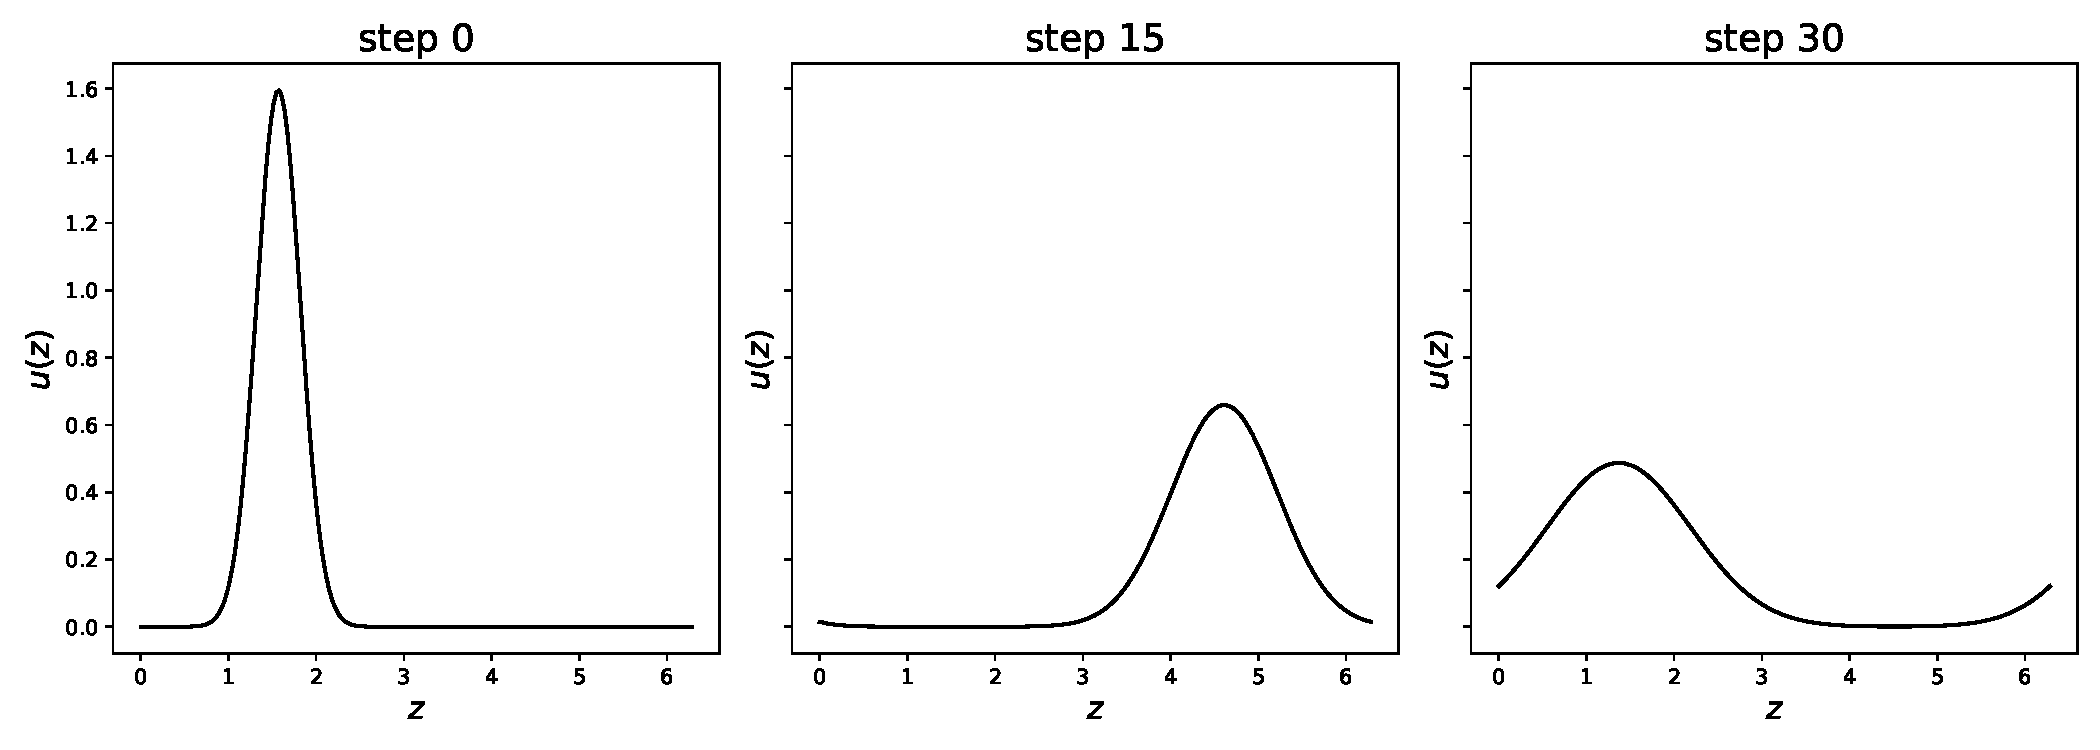
\includegraphics[width=\linewidth]{images/app1d/analytical_frame.pdf}
	\caption{The analytical solution of the convection-diffusion problem evolves over time, with the final snapshot revealing a complete spatial period.}
	\label{fig:1d_analytical}
\end{figure}

Following a Lagrangian perspective by tracking a fluid particle of position $z_p$ and intensity $U_p$, the equation becomes

\begin{equation*}
	\frac{dz_p}{dt} = v(z_p, t), \quad \frac{dU_p}{dt} = D \frac{d^2 U_p}{dz^2}
\end{equation*}

To solve the convection-diffusion scheme, we employ the two steps of the viscous splitting algorithm. The advection is taken into account by updating the position of the particle with an Euler explicit scheme.
On the other hand, we use a redistribution method called the Particle Strength Exchange Method (PSE)~\cite{degond_1989,cottet_1990} to approximate the laplacian term $\frac{d^2 U_p}{dz^2}$.


\begin{equation*}
	D \frac{d^2 U_p}{dz^2}  = D V_p \frac{d^2 u_p}{dz^2} \approx D V_p \varepsilon^{-d} \int [u(z)  - u(y)] \phi_\varepsilon(y - z) dz,
\end{equation*}

It deals with the particle approximation by a redistribution of the particle intensities in their previous locations, such as

\begin{equation*}
	\frac{dU_p}{dt} = D \varepsilon^{-d} V_p \sum_q (U_q - U_p) \phi_\varepsilon( z_q -  z_p),
\end{equation*}where $V_p$ the volume of the particle $p$ and $d$ the dimension of $\Omega$.
For further details on the computation, please refer to \cite{cottet_1990}.

For the periodic boundary problem described in section \ref{App_1D}, we define an equivalent kernel function $\phi_\varepsilon= \phi^P_g = \sum_{n=-\infty}^{+\infty} \phi_g(r - 2 \pi  n )$.

The particle-based model employs a discretization of \npart{} particles with a size of $h = \frac{L}{N_{\text{part}}}$ and a smoothing length of $\varepsilon = 1.3 h$.
For the sake of comparison, we solve the convection-diffusion equation with an explicit central finite difference scheme discretized on a regular grid with \ngrid{} nodes.

\subsection{Assimilation parameters and ensemble generation}

\subsubsection{Ensemble distribution}
All filters undergo testing on an identical initial prior ensemble of size $N = 25$ members, characterized by Gaussian shapes that are shifted and scaled. The mean of the function and its standard deviation are sampled. The total mass is set equal to 1. Parameters of velocity $v$ and the diffusion $D$ are also sampled. The different distributions are defined in Appendix~\ref{tab:ens_gen_1d}. Moreover, the parameters samples and initial state are illustrated in Figure~\ref{fig:initial_gen}.

The observational data is subject to additive noise, denoted as $\eta \sim \mathcal{N}(0, \sigma_y \bm{I})$, where $\sigma_y = \sigmaY$ and $\bm{I}$ represents the identity matrix.

\subsubsection{Error definition}
We define the error as the following relative ratio

\begin{equation}~\label{eq:L2_error}
	e_{L_2} =\frac{ \left[\frac1\nens \sum_{i = 1}^{\nens} \int_\Omega \left(u_i(z) - u^{gt}(z)\right)^2 dz\right]^{1/2}}{\norm{u^{gt}}_{L_2}}
\end{equation}~where $u_i$ denote the $i$-th member of the ensemble and $\norm{u}_{L_2}$ denote the $L_2$ norm of $u^{gt}$.

The $L_2$ norm is computed using a quadrature over a regular grid of an ensemble of cells $\mathcal{C}$ such as for any $f \in L_2$

$$
	\norm{f}_{L_2}  = \int_{\Omega} f^2~d\Omega \approx \sum_{c \in \mathcal{C}} f(z)~V_c
$$~where $z_c$ is the center of the cell $c$ and $V_c$ the volume of the cell. The grid is still the same for all the simulations.
%We compute the parameter error with a norm-2 as $e_{\theta} = \frac{ \left[\frac1\nens \sum_{i = 1}^{\nens} \norm{\theta^{gt} - \theta_{i}}_2^2\right]^{1/2}}{\norm{\theta^{gt}}_2}$.

\subsubsection{Numerical parameters}

We conduct $N_{\text{assim}} = 30$ assimilation steps at evenly spaced intervals until the final time $t_f = 2 \frac{L}{v}$. During each assimilation step, the field $u^{gt}$ is observed at six regularly spaced positions $x_{\text{obs}}$.


In the particle-based simulation, fields are discretized using regularly spaced particles that are shifted. Intensity values are obtained by fitting an interpolation operator like in Section~\ref{interpOp} to the particle intensity.
The parameter $\varepsilon_{\text{mass}}$ is introduced as a cutoff for particle selection, allowing for the definition of varying numbers of particles for each simulation. The particle support poses challenges in the Part-EnKF as described in Section \ref{part_enkf}.

Simultaneously, a standard Ensemble Kalman Filter (EnKF) update is applied to the nodal variables to construct the reference filter Grid-EnKF, which uses a grid-based model. For grid-based simulation, the fields of each member are interpolated at the node locations. In this way, the ensemble generated is still the same for the sake of comparison.


\begin{figure}[ht!]
	\centering
	\begin{subfigure}{0.49\textwidth}
		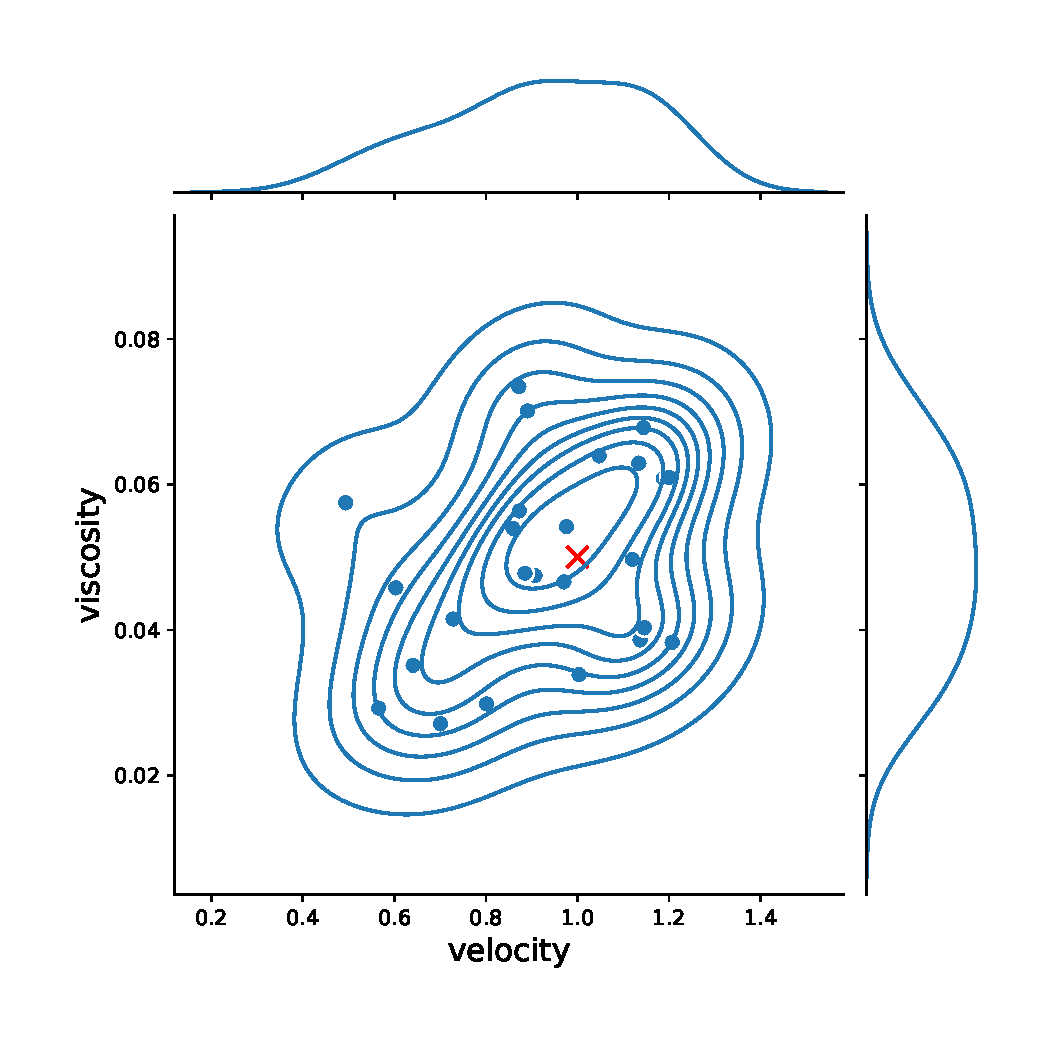
\includegraphics[width=\textwidth]{images/app1d/param.pdf}
	\end{subfigure}
	\hfill
	\begin{subfigure}{0.49\textwidth}
		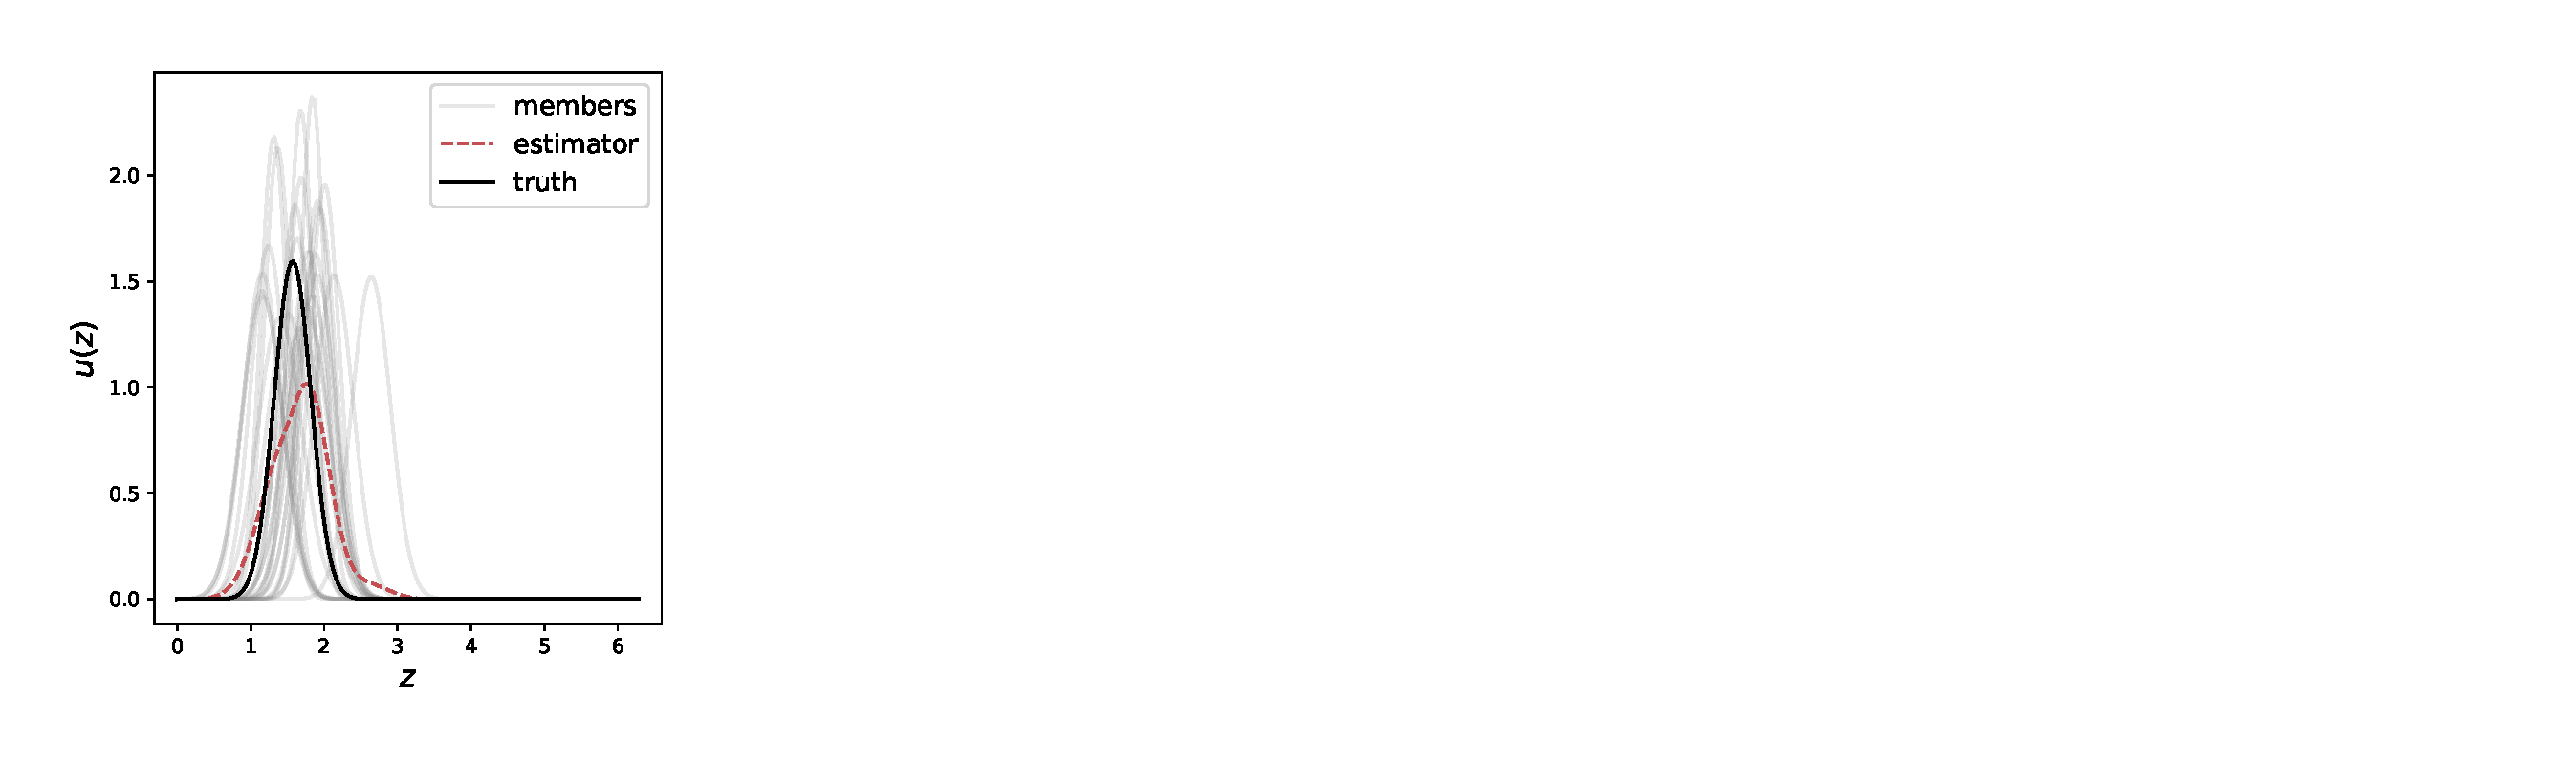
\includegraphics[width=\textwidth]{images/app1d/prior.pdf}
	\end{subfigure}
	\caption{On the left the initial parameters sample, $v$ in abscissa and $D$ in ordinate. On the right is the initial ensemble state.}
	\label{fig:initial_gen}
\end{figure}

\subsection{Results}

We compare the different filters on the assimilation of the state. We first compare the Grid-EnKF, the Remesh EnKF, and two Part-ENKF filters with 100 and 60 particles. The parameter sample is still unchanged. We take unknown parameters into account as model uncertainties. The two filters outlined in the Method section~\ref{Methods} and the Eulerian filter are compared with the reference filter based on a grid discretization.

In figure \ref{fig:1d_error_time}, we appreciate different assimilation steps for the Remesh-EnKF filter.


\begin{figure}
	\centering
	\begin{subfigure}{\textwidth}
		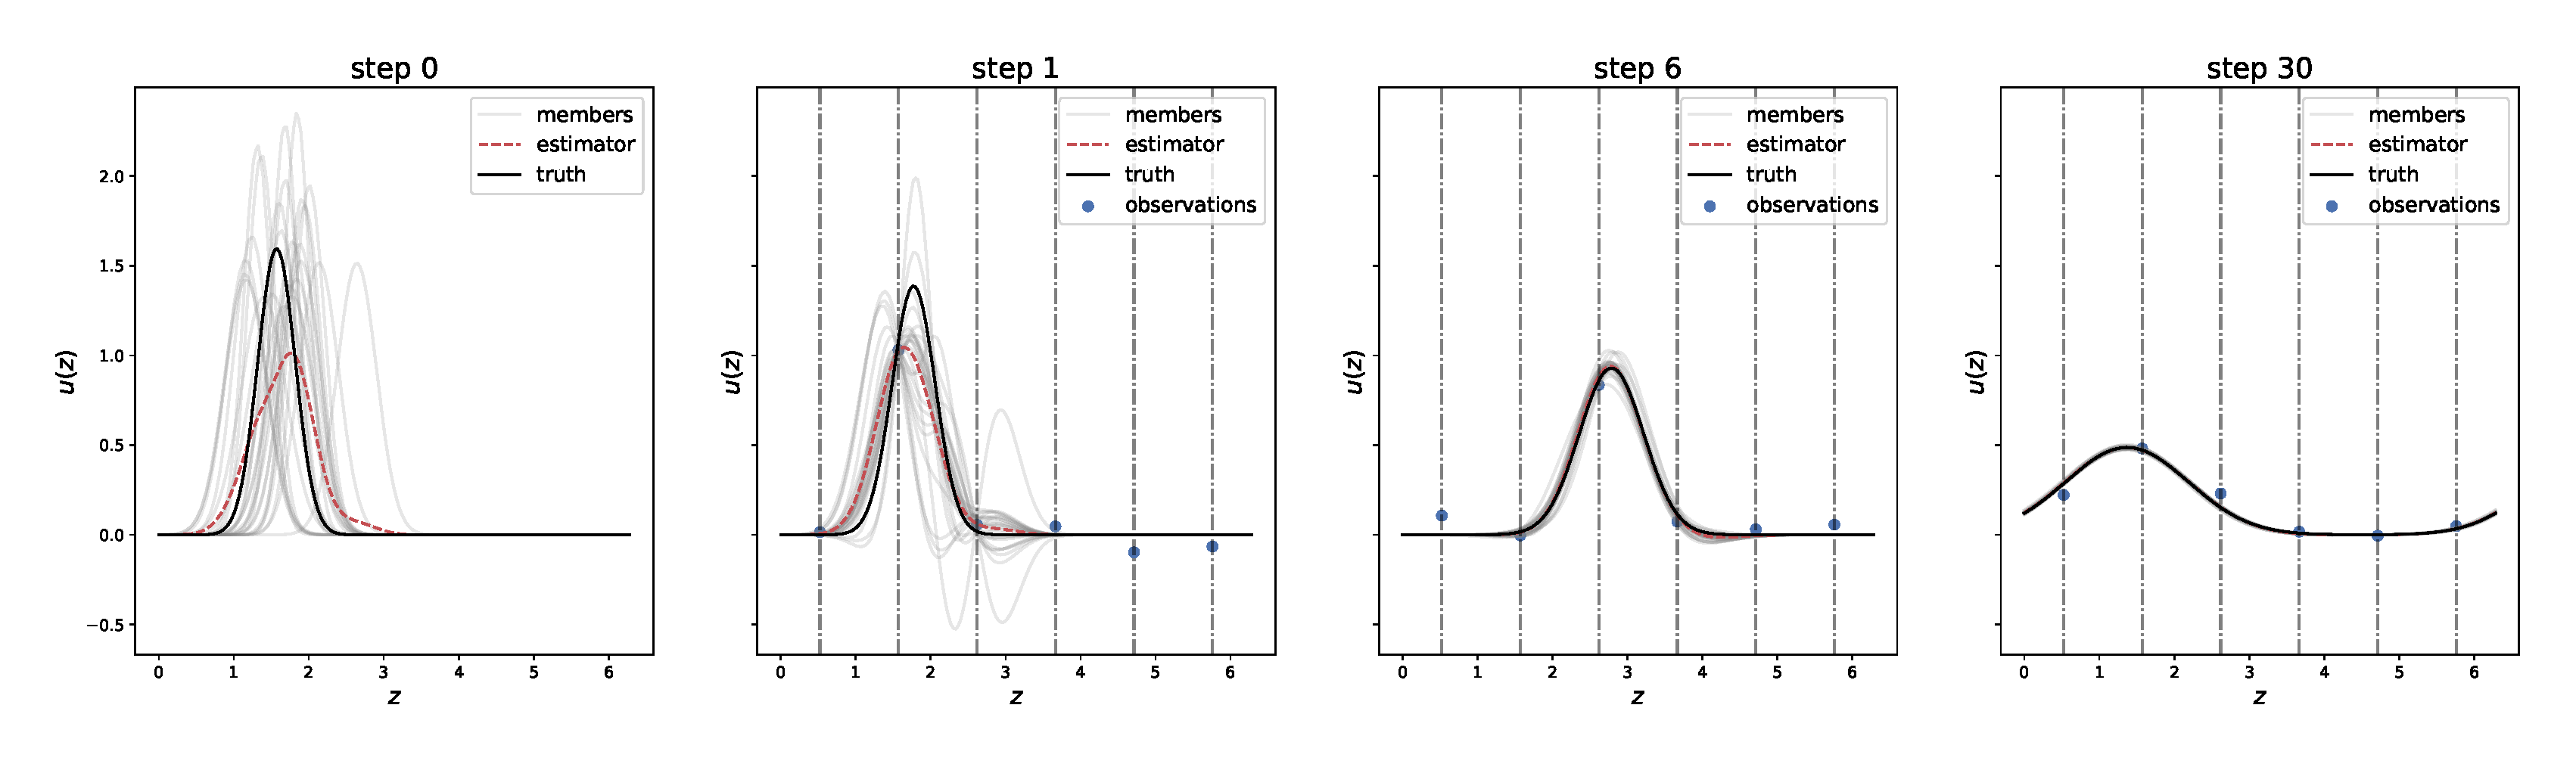
\includegraphics[width=\textwidth]{images/app1d/wo_calibration/remesh_EnKF.pdf}
	\end{subfigure}
	\caption{Data assimilation ower assimilation step for the Remesh-EnKF filter.}
\end{figure}

The result is quite similar for all the different filters except the Part-EnKF with 60 particles.

\begin{figure}
	\centering
	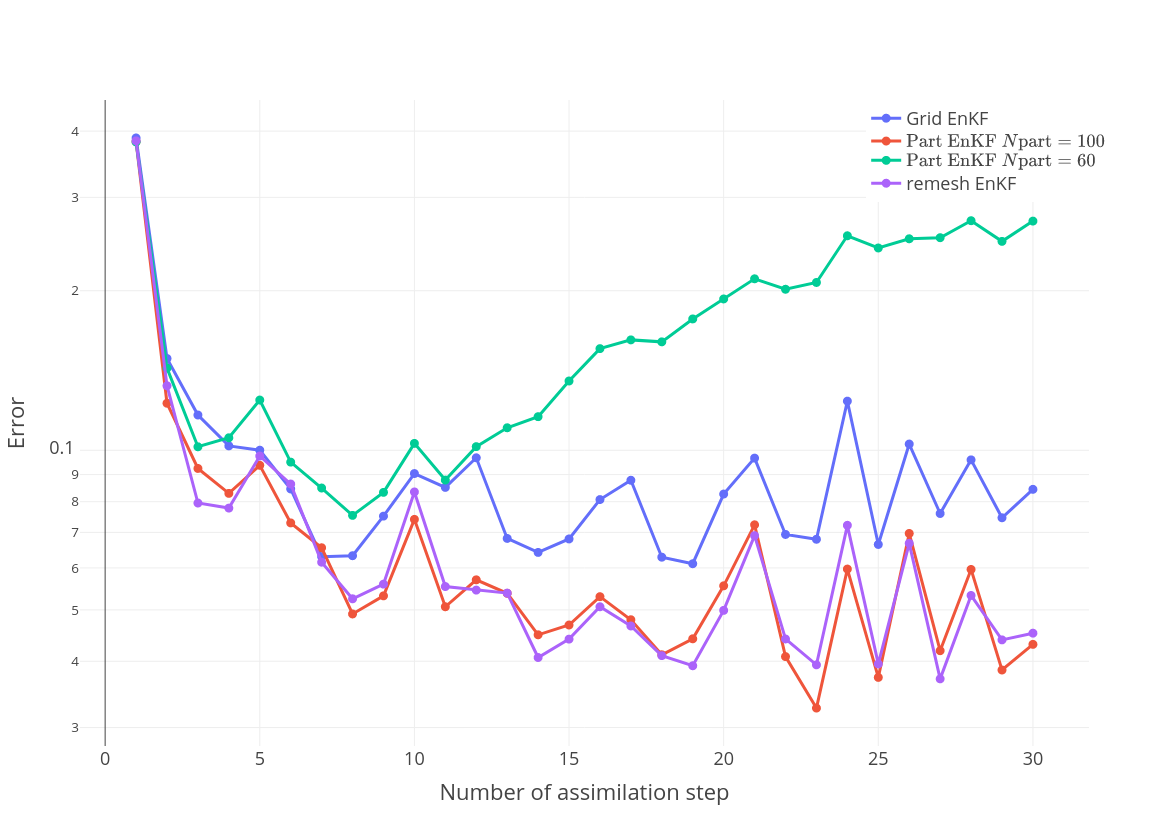
\includegraphics[width=0.75\textwidth]{images/app1d/wo_calibration/state_error.png}
	\caption{State error with respect to assimilation time step.}
	\label{fig:1d_error_time}
\end{figure}

The primary issue arises from the regression on non-overlapping support, where the regression struggles to fit the analysis solution defined on a more considerable space support. This leads to heightened variability, particularly in the tail of the distribution. Addressing this common challenge in RBF Regression \cite{fornberg_flyer_2015} involves increasing the Ridge penalization coefficient, a parameter we choose through cross-validation Ridge regression.
Even with a more stable regression, it remains a projection of the analysis solution onto the forecast support. It is imperative to increase the number of particles to achieve a better approximation of the analysis solution using the particle approximation operator in Section~\ref{interpOp} or the regression operator in Section~\ref{regressionOperator}.

We validate this assumption by varying the initial support of particles. Quantitatively, as observed in Figure~\ref{error_support}, the error estimate and dispersion decrease with an increase in the number of particles. At the level of 70 particles support, a threshold is reached. Moreover, qualitatively examining the snapshot on the right reveals that the solution closely aligns with the reference.

\begin{figure}
	\centering
	\begin{subfigure}{0.39\textwidth}
		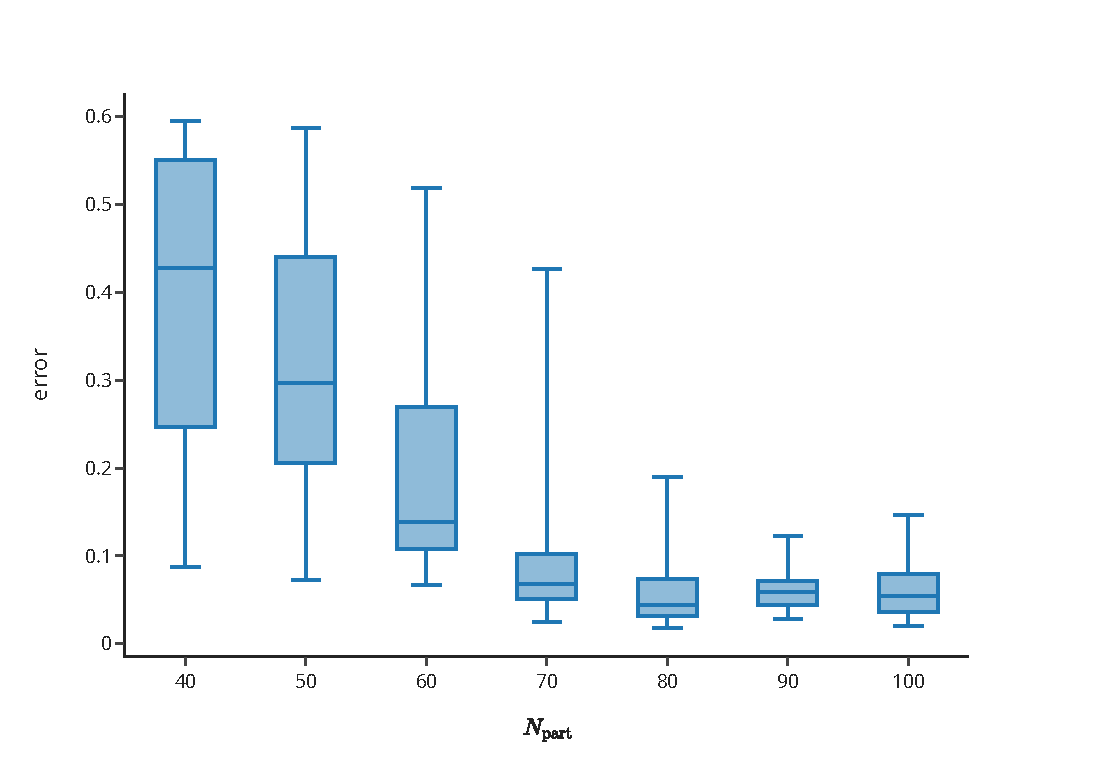
\includegraphics[width=\textwidth]{images/app1d/error_support/error_part.pdf}
		\label{error_support1}
	\end{subfigure}
	\hfill
	% Revoir figures en plotly
	\begin{subfigure}{0.29\textwidth}
		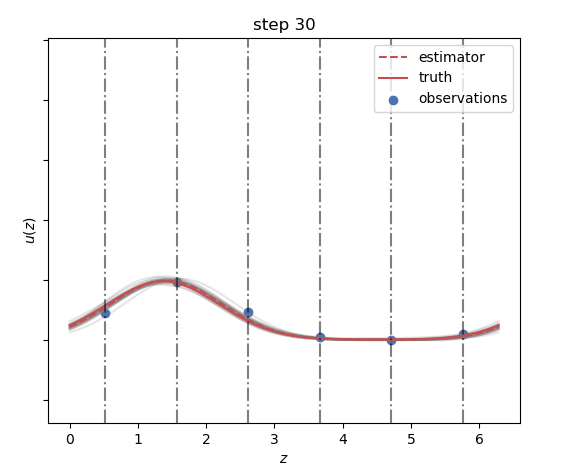
\includegraphics[width=\textwidth]{images/app1d/error_support/ok.png}
		\label{error_support2}
	\end{subfigure}
	\hfill
	\begin{subfigure}{0.29\textwidth}
		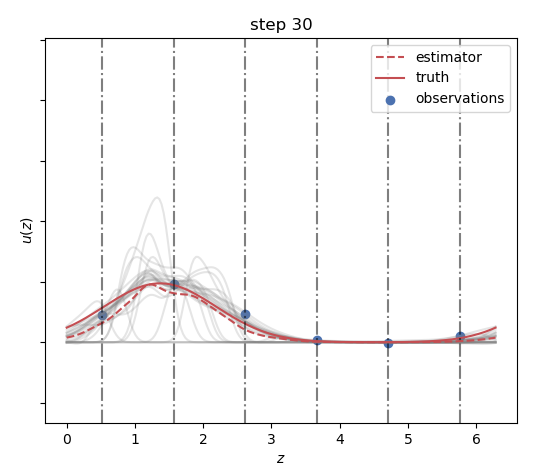
\includegraphics[width=\textwidth]{images/app1d/error_support/not_ok.png}
		\label{error_support3}
	\end{subfigure}
	\caption{Left: Error with respect to particle support size, Middle: Final step for a support of 100 particles, Right: Final step for a support of 60 particles.}
	\label{error_support}
\end{figure}
However, Adding particles to a more complex solution is challenging. Indeed, good spacing between particles and particle density has to be preserved. In this case, we advise defining criteria for the reconstruction' error. Instead of adding particles, we advise generating a new, regularly spaced grid of particles to reconstruct the solution.

In conclusion, this example underscores the Remesh-EnKF filter capability to yield results comparable to the classical EnKF applied to a grid model. Additionally, it highlights the Part-EnKF capability in assimilating on a particle discretization while also emphasizing the importance of addressing spatial discrepancies between members, which can pose challenges in solution reconstruction. The computation of solution error reconstruction provides a straightforward criterion for remeshing a member and applying the analysis solution approximation.


\newpage
% !TEX root = main.tex

\section{2D vortex-in-cell problem}~\label{App_2D}
\subsection{Description of the method}


In this section, we apply the Vortex Method in a two-dimensional scenario, as outlined by Cottet et al. \cite{cottet_vortex_2000}. The Vortex Method is a Lagrangian approach utilizing a particle ensemble to discretize the vorticity field, allowing for the solution of the Navier-Stokes equation for viscous incompressible flow. The method is grounded in the vorticity-velocity formulation of the Euler equation, where $\bm \omega = \nabla \times \bm{v}$ satisfies

\[
	\begin{aligned}
		\frac{\partial \bm \omega}{\partial t} + (\bm{v} \cdot \nabla) \bm \omega - \nu \Delta \bm \omega & = 0, \\
		\nabla \cdot \bm v                                                                                & = 0,
	\end{aligned}
\]where $\omega$ denotes vorticity, $\bm{v}$ represents velocity, and $\nu$ stands for viscosity.

In the context of 2D flow, vorticity is perpendicular to the flow plane, forming a scalar field denoted as $\omega$. In Cartesian coordinates, it is expressed as $\omega = \frac{\partial v_y}{\partial x} - \frac{\partial v_x}{\partial y}$.

The vorticity field is discretized using a collection of discrete vortices, each characterized by a position $\bm z_p$, an associated kernel $\phi_\varepsilon$, and a circulation $\Gamma_p$. For all points $\bm z$ within the domain $\Omega$, the vorticity is expressed as

\begin{equation*}
	\omega(\bm z) = \sum_{i=1}^{N_p} \Gamma_p \phi_\varepsilon(\bm z - \bm z_p).
\end{equation*}

To address the Navier-Stokes equation, we employ a viscous splitting scheme, following the methodology outlined in \cite{cottet_1990}, acknowledging the predominance of the convection term over viscosity. We use the Vortex-In-Cell algorithm \cite{christiansen_1973, birdsall_1969}, coupled with an FFT solver to compute the advection velocity. The subsequent steps involve assigning particle vorticity values to the grid using a particle-to-grid formula and computing the velocity field by solving the Poisson equation on the grid verified by the stream function. Finally, the velocity is interpolated back onto the particles using the grid-to-particles formula. A Runge-Kutta 3 time-stepping scheme is employed to update the particle positions through a time integration scheme. The final phase involves solving the heat equation and updating the particle intensities thanks to the PSE method previously described in Section~\ref{App_1D}.

\subsection{Lamb-Chaplygin dipole and simulation parameters}

We define the reference as the advection of the Lamb-Chaplygin dipole inside a close domain with stress-free walls. Lamb-Chaplygin dipole is a popular choice for numerical studies \cite{orlandi_vortex_1990}. The model represents a specific steady, inviscid dipolar vortex flow and offers a non-trivial solution to the two-dimensional Euler equations. The dipole is characterized by a translation velocity $U$, a mean position $\bm{z}_0$, a radius $R$, and an orientation $\alpha$.

The dipole vorticity field $\omega$ could be expressed as

\begin{equation*}
	\omega(r) = \begin{cases}
		\frac{-2 k U J_1(kr)}{J_0(kR)} \sin \alpha \quad & \text{for} \quad  r < R, \\
		0 \quad                                          & \text{otherwise},
	\end{cases}
\end{equation*}where $(r, \alpha)$ represent the polar coordinates in the dipole reference frame. Here, $J_0$ and $J_1$ denote the zeroth and first-order Bessel functions of the first kind, respectively, and $k$ is determined such that $kR$ corresponds to the first non-trivial zero of the first Bessel function. The dipole vorticity field is depicted in Figure \ref{fig:lamb_dipole}.

\begin{figure}[ht]
	\centering
	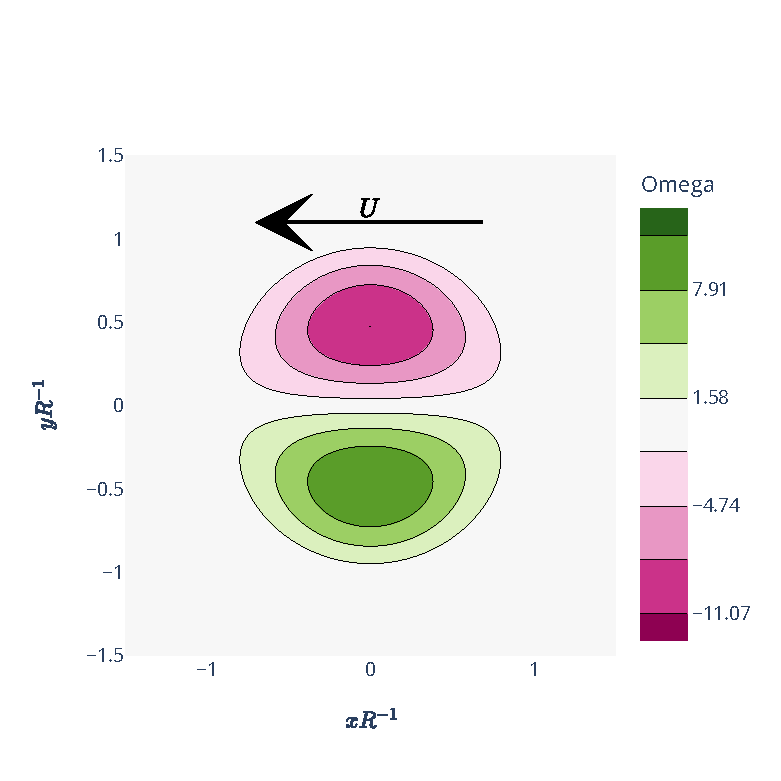
\includegraphics[width=0.6\linewidth]{images/app2d/lamb.pdf}
	\caption{The Lamb-Chaplygin dipole vorticity field on a normalized space.}
	\label{fig:lamb_dipole}
\end{figure}

The dipole is positioned at the center of a box with dimensions $[0, \pi] \times [0, \pi]$, featuring an orientation of $\frac{7\pi}{8}$ rad., a radius of $0.5$ meters, and a velocity $U$ of $0.25 \text{ m.s}^{-1}$. The complete reference setting is listed in Table \ref{tab:ref}.

The boundary box features stress-free walls, meaning fluid cannot pass through them. The velocity perpendicular to the walls is zero, while tangential velocity remains undetermined. When a vortex, such as a dipole, reaches this boundary, it walks along the wall, sensing its reflection and interacting with it.

Because this problem does not have an explicit solution on a closed domain, we simulate the ground truth with the vortex method for a fined discretization and fixed set of parameters also described in Table \ref{tab:ref}. The trajectory of the ground truth is illustrated in Figure \ref{fig:ref_trajectory} on a regularly spaced grid.

\begin{figure}[htbp]
	\begin{subfigure}{0.32\textwidth}
		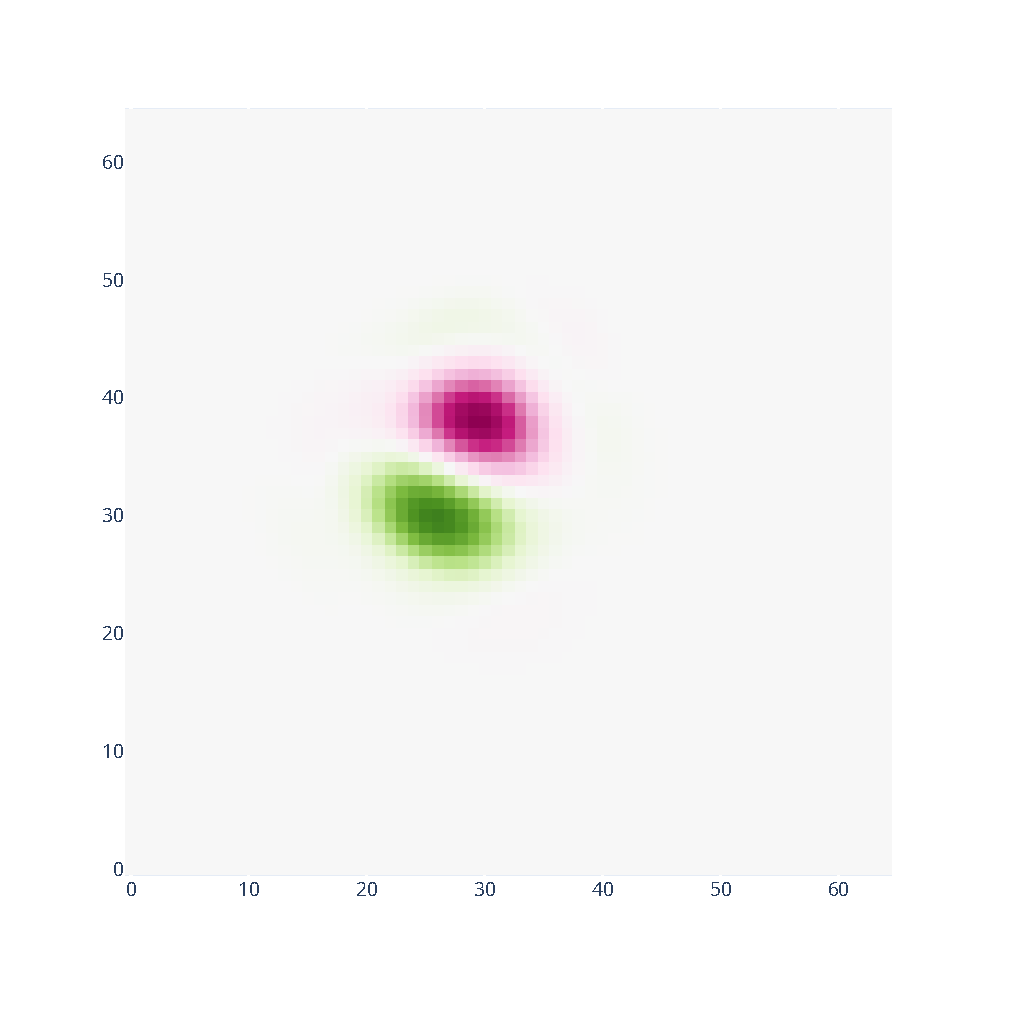
\includegraphics[width=\linewidth]{images/app2d/best_estimate_2.pdf}
	\end{subfigure}
	\hfill
	\begin{subfigure}{0.32\textwidth}
		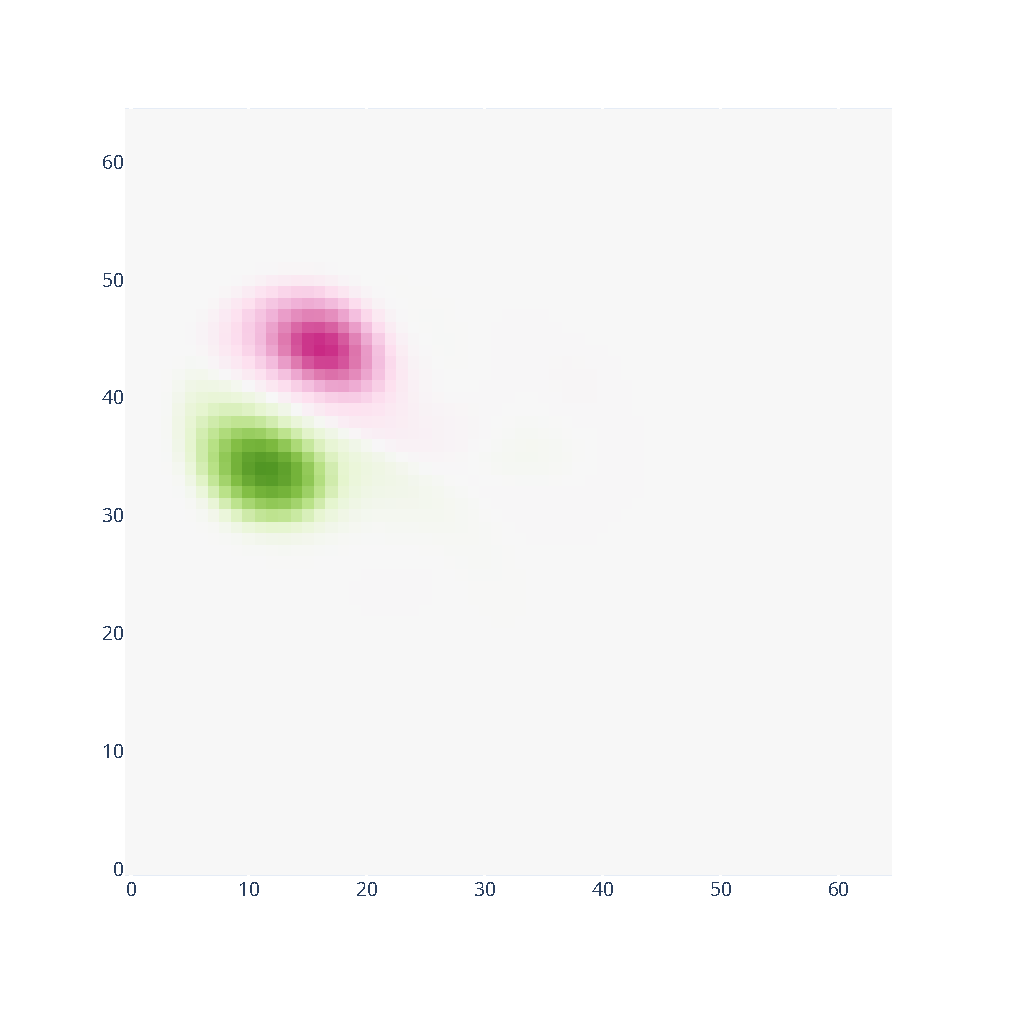
\includegraphics[width=\linewidth]{images/app2d/best_estimate_10.pdf}
	\end{subfigure}
	\hfill
	\begin{subfigure}{0.32\textwidth}
		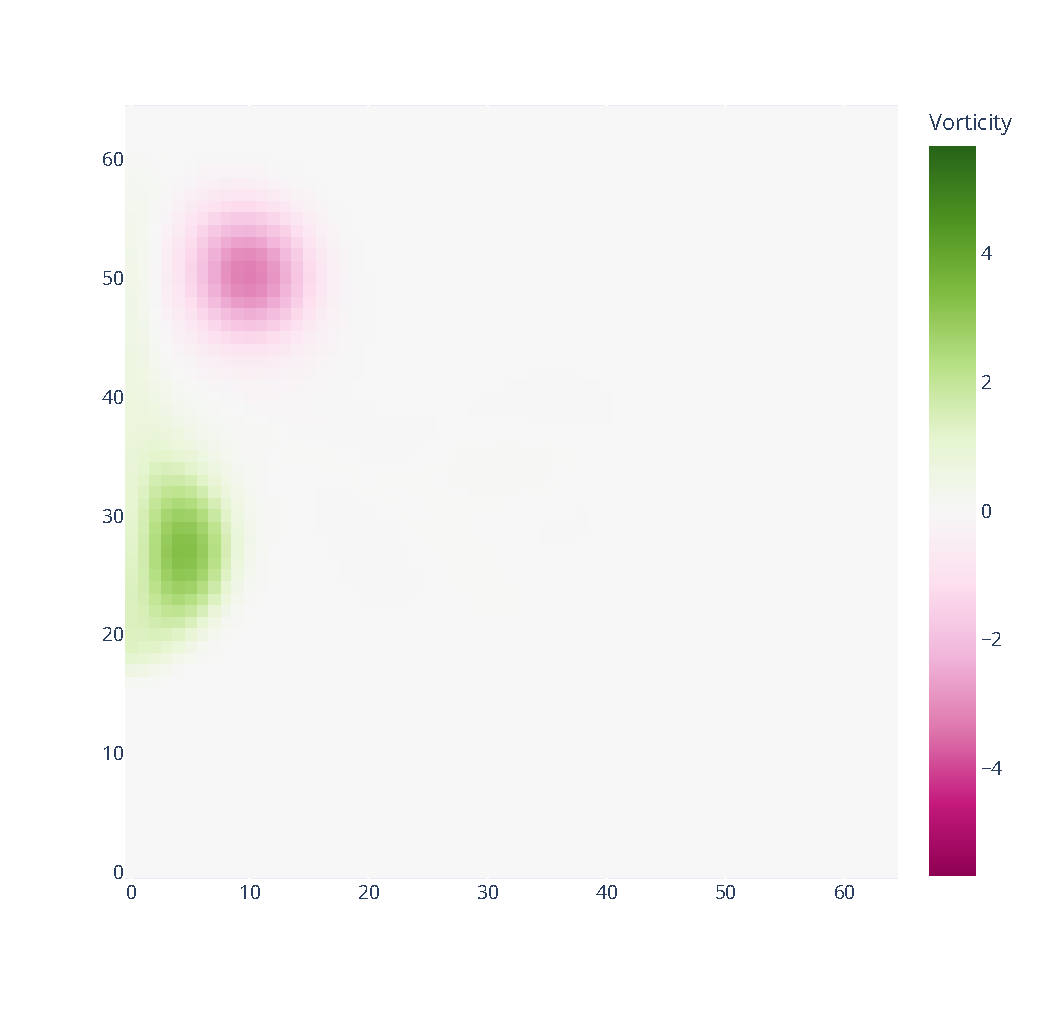
\includegraphics[width=\linewidth]{images/app2d/best_estimate_20.pdf}
	\end{subfigure}
	\caption{Trajectory of the ground truth. The vorticity is represented on a regularly spaced grid. For $t=[1, 5, 10]s.$}
	\label{fig:ref_trajectory}
\end{figure}
Several parameters in the simulation influence the particle distribution and can lead to different results. The first one is the particle size defined by $d_p$. Another significant parameter is $\varepsilon_\omega$, associated with the remeshing process occurring either during the forecast (to prevent high distortion of the particle distribution) or during the Remesh-EnKF filter. $\varepsilon_\omega$ serves as a threshold, determining whether a particle is retained after the remeshing process based on the condition $V_p \Gamma_p > \varepsilon_\omega$. The impact of this parameter is illustrated for one member after the first forward in Figure~\ref{fig:eps_effect}.

\begin{figure}[htbp]
	\centering
	\begin{subfigure}{0.3\textwidth}
		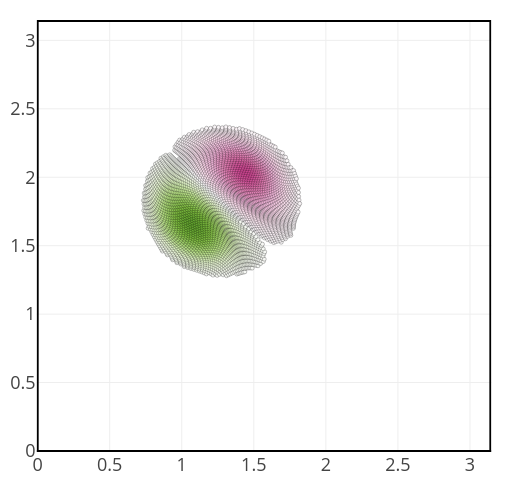
\includegraphics[width=\linewidth]{images/app2d/part_eps_0.1.png}
	\end{subfigure}
	\hfill
	\begin{subfigure}{0.3\textwidth}
		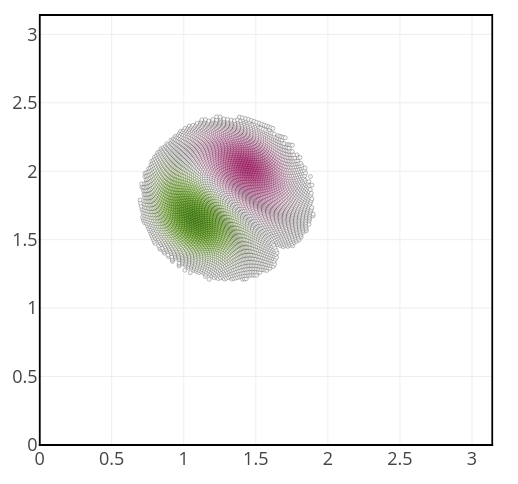
\includegraphics[width=\linewidth]{images/app2d/part_eps_0.01.png}
	\end{subfigure}
	\hfill
	\begin{subfigure}{0.3\textwidth}
		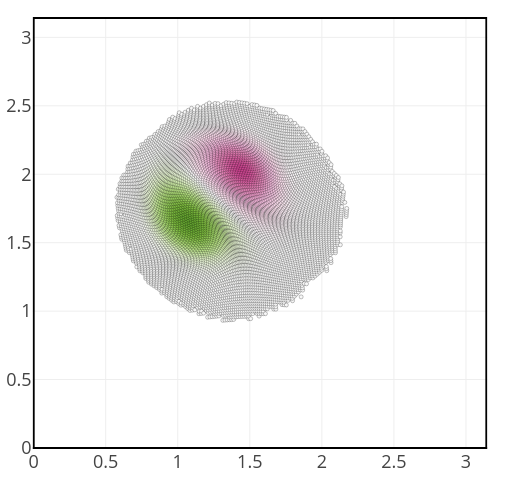
\includegraphics[width=\linewidth]{images/app2d/part_eps_1e-6.png}
	\end{subfigure}
	\caption{Effect of the parameter $\varepsilon_\omega$ on the particle discretization of the solution for one member. From left to right, results for $\varepsilon_\omega = 0.1, 0.01$, and $1.e^{-6}$.}
	\label{fig:eps_effect}
\end{figure}

For the following paragraphs, if the value is not explicitly changed, we use the nominal parameters described in Table \ref{tab:simu_2d} for the simulation.

\subsection{Assimilation parameters and ensemble generation}

\subsubsection{Ensemble distribution}
An ensemble of 32 members is created by sampling distributions over the dipole parameters. We sample the radius $R$, the prescribed velocity $U$, the orientation $\alpha$, and the barycenter $\bm z_{\text{mean}}$. Additionally, the model viscosity $\nu$ is also sampled. All the distributions are summarized in Table \ref{tab:ens_dipole}. The first six members are plotted in Figure \ref{fig:sample_ens}.

\begin{figure}[ht]
	\centering
	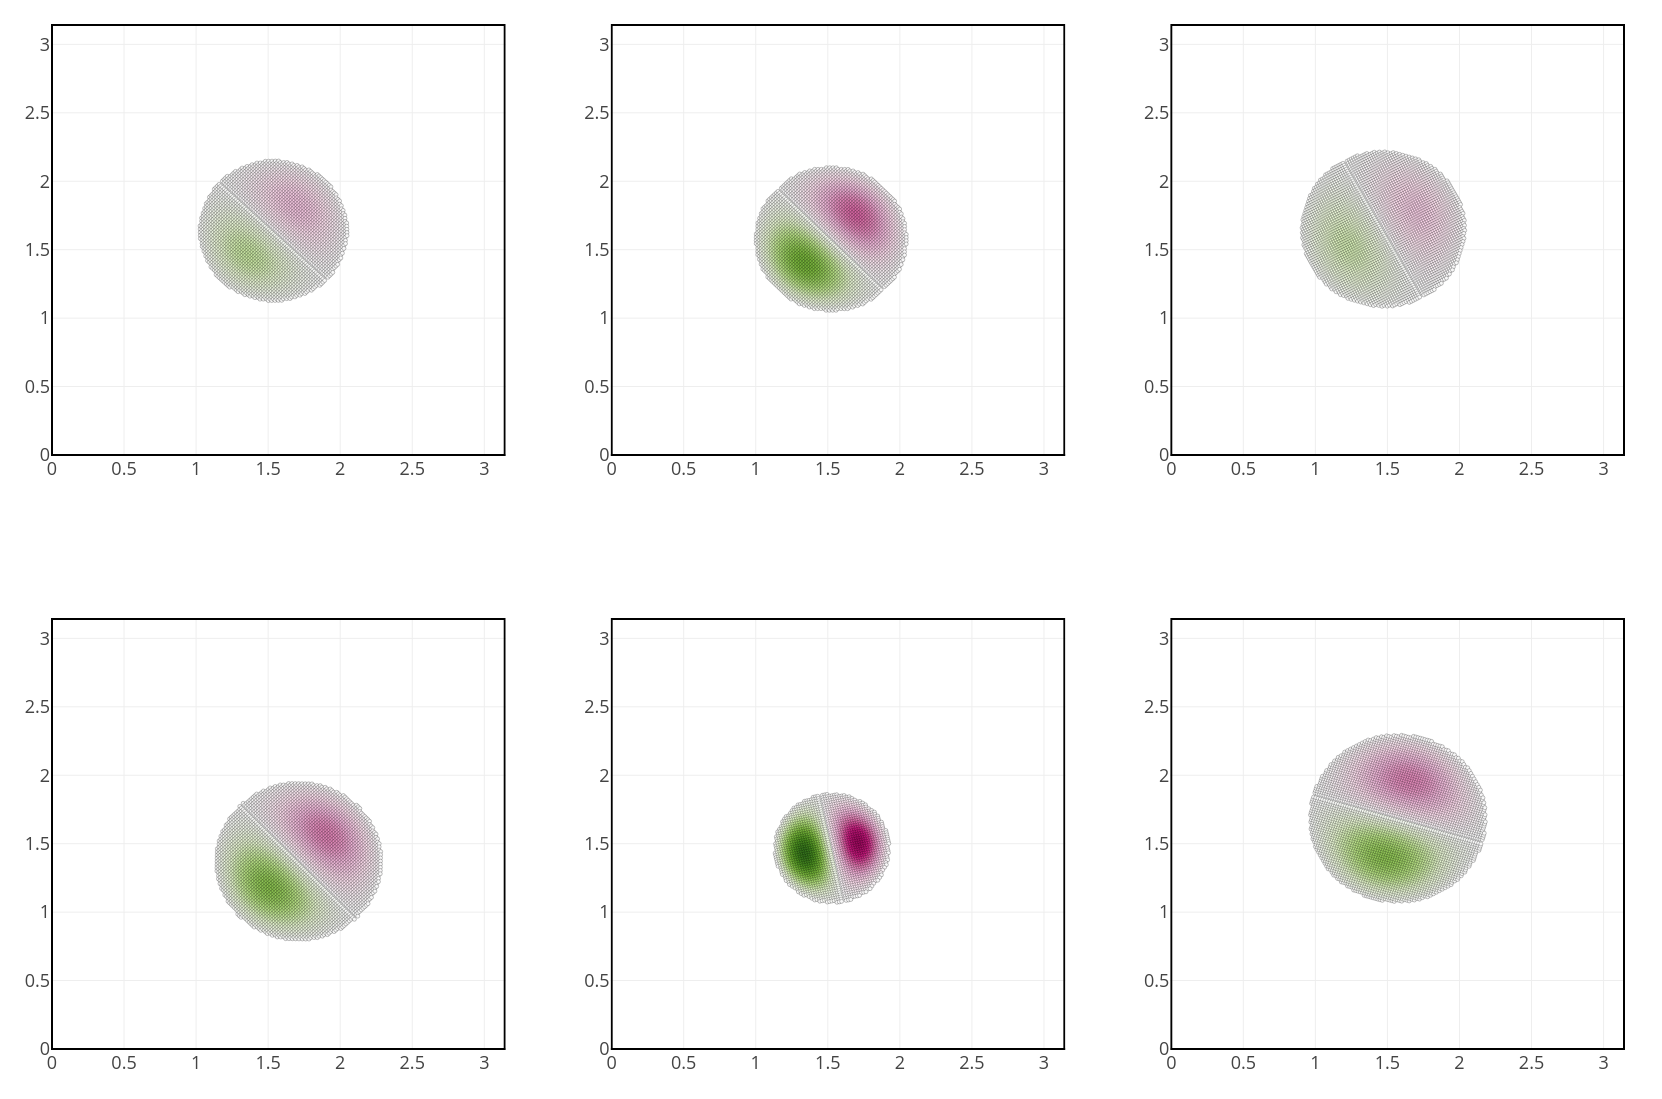
\includegraphics[width=0.9\linewidth]{images/app2d/ensemble_sample.png}
	\caption{Six samples from the initial ensemble.}
	\label{fig:sample_ens}
\end{figure}

The initial vorticity field is first discretized on a regular grid of particles with a characteristic length $d_p$, where each particle receives the circulation $\Gamma_p = \omega(\bm z_p) V_p$ and $V_p = d_p^2$ represents the volume of the particle.

\subsubsection{Error definition}

We use an absolute error absolute \(L_2\)-error defined as $ \frac1\nens \sum_{i = 1}^{\nens} \int_\Omega \left(\omega_i(\z) - \omega^{gt}(\z)\right)^2 \mathrm{d}\z$.
We also use the member errors to evaluate the dispersion of the error estimate.

\subsubsection{Numerical parameters}

The assimilation frequency is defined by the assimilation step $dt_a$. The simulation is performed over a duration of $t_f$. All simulation parameters are summarized in Table \ref{tab:simu_2d}.

Observations are collected on a regular grid of size $N_{\text{obs}}$, measuring both components of the velocity. The observations follow a normal distribution $\mathcal N(0, \sigma_{\text{obs}}^2 \bm{I})$, indicating an ensemble of independent measurements, each characterized by a standard distribution of $\sigma_{\text{obs}}$. An example of observed velocity with and without noise is illustrated in Figure \ref{fig:velocity}.

\begin{figure}[htbp]
	\centering
	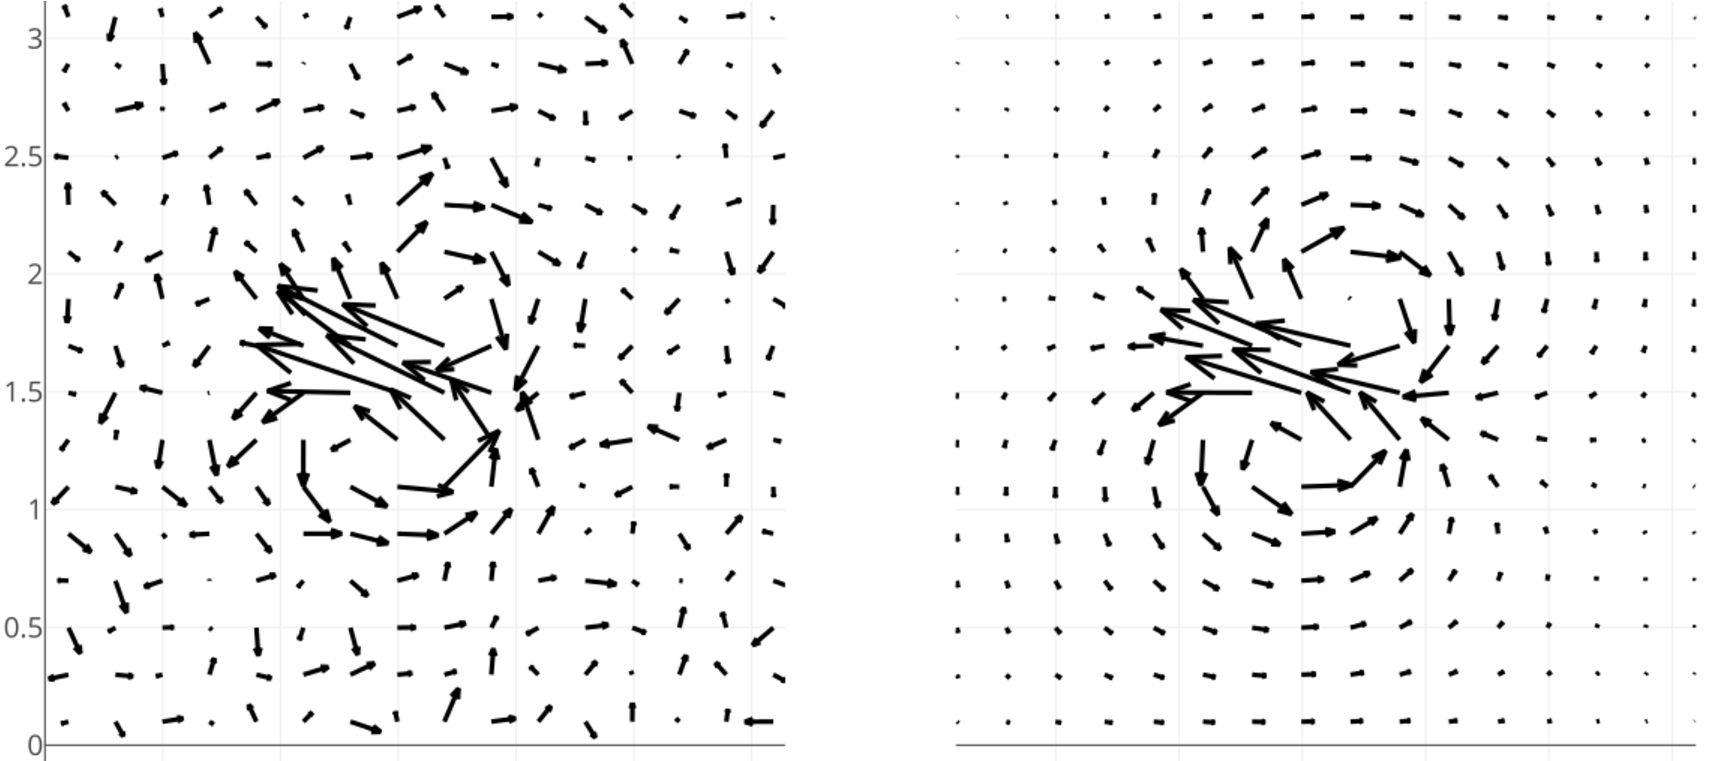
\includegraphics[width=0.8\linewidth]{images/app2d/velocity_ref_recadre.pdf}
	\caption{Observed and reference velocity fields. The error on each component is a sample from a centered normal distribution with the nominal value $\sigma_{\text{obs}} = 0.05$.}
	\label{fig:velocity}
\end{figure}

\newpage

\subsection{Results}

\subsubsection{Error through time}

We start by analyzing the assimilation error over time. Figure \ref{fig:assim_time} illustrates the error throughout the assimilation process for the nominal set of assimilation parameters, demonstrating comparable results for both filters. At each assimilation step, the error decreases and prevents the solution from diverging elsewhere.

\begin{figure}[htbp]
	\centering
	\includegraphics*[width=0.7\linewidth]{images/app2d/final/error_in_time.pdf}
	\caption{error curves through assimilation steps. Left: \(L_2\)-error of the field, Right: Error for the viscosity parameter. With Part-EnKF in blue and Remesh-EnKF in red.}
	\label{fig:assim_time}
\end{figure}

\newpage

\subsubsection{Error with respect to assimilation parameters}
We also assess the performances of the different filters by evaluating the convergence of the error with respect to the assimilation parameters.

We observe the convergence rate concerning data assimilation parameters: The observation precision, which is \(1/\sigma_{\text{obs}}^2\), the number of observations \(N_{\text{obs}}\), the number of assimilation step \(N_{\text{assim}}\).

Figure \ref{fig:obs_precision_1} illustrates a decreasing error bias and variances with respect to observation precision similarly for both filters. What is striking in the same Figure~\ref{fig:obs_precision_2} but in the log-scale is the regular convergence rate for both filters with respect to the observation precision. The order of convergence is about 0.68 for Part-EnKF and 0.75 for Remesh-EnKF.

\begin{figure}[h!]
	\centering
	\begin{subfigure}{0.49\linewidth}
		\centering
		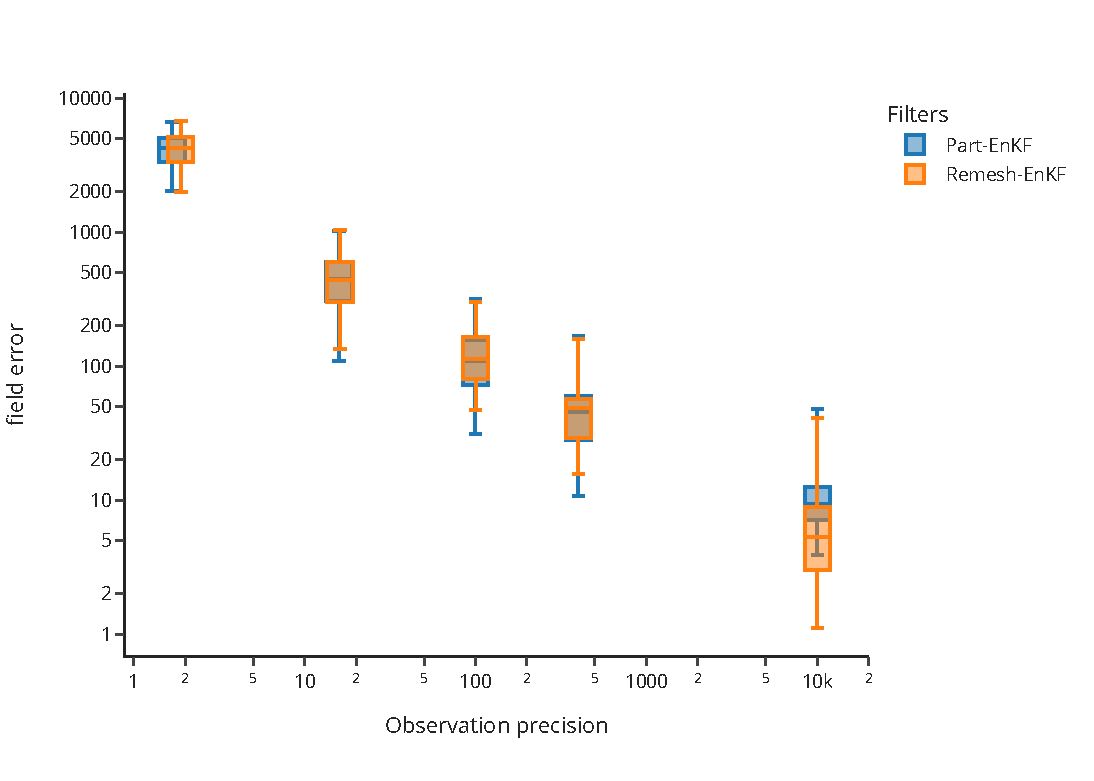
\includegraphics[width=\linewidth]{./images/app2d/final/MSE_obs_precision_box.pdf}
		\caption{}
		\label{fig:obs_precision_1}
	\end{subfigure}
	\begin{subfigure}{0.49\linewidth}
		\centering
		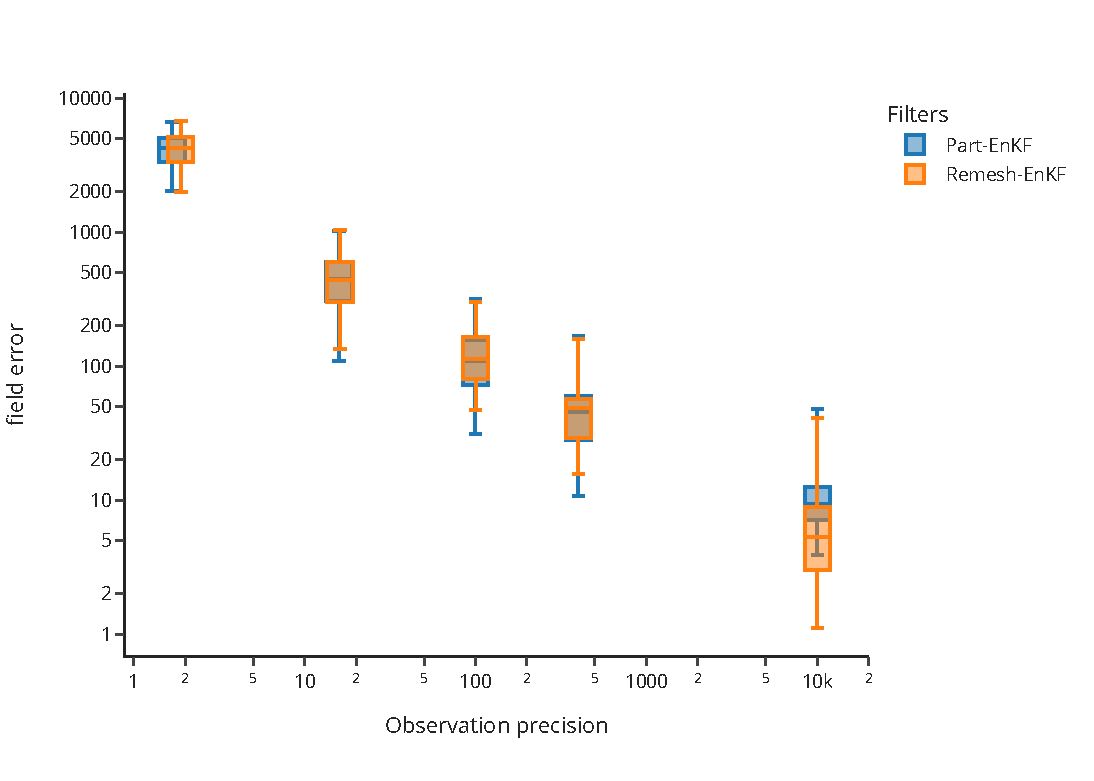
\includegraphics[width=\linewidth]{./images/app2d/final/MSE_obs_precision_box_log.pdf}
		\caption{}
		\label{fig:obs_precision_2}
	\end{subfigure}
	\caption{Box plots of the state error w.r.t. $1/\sigma_{\text{obs}}^2$.}
\end{figure}


In Figure~\ref{fig:na_1}, the reduction of error is still prominent and shows a reduction of variance as the number of observations increases. In the log-scale Figure~\ref{fig:na_2}, the error decrease also at a constant rate for both filters. We notice a more substantial order of 1.8 for the Remesh-EnKF compared to an order of 1.4 for Part-EnKF.

\begin{figure}[h!]
	\centering
	\begin{subfigure}{0.49\linewidth}
		\centering
		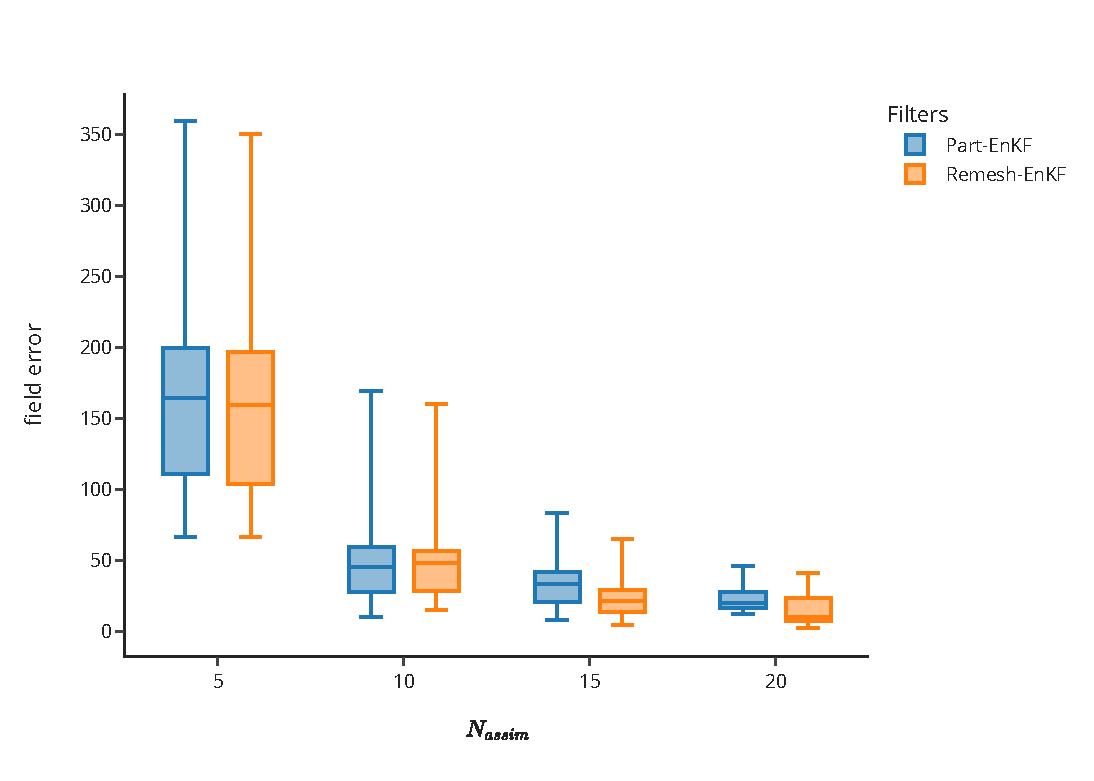
\includegraphics[width=\linewidth]{./images/app2d/final/MSE_na_box.pdf}
		\caption{}
		\label{fig:na_1}

	\end{subfigure}
	\begin{subfigure}{0.49\linewidth}
		\centering
		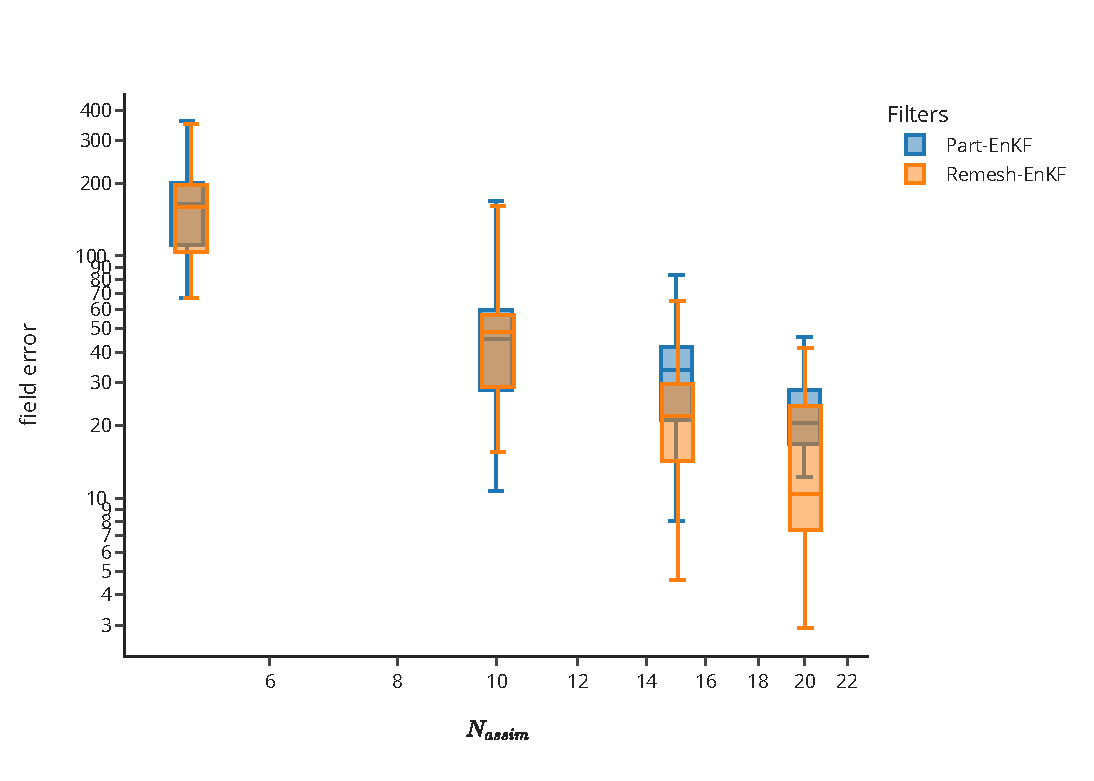
\includegraphics[width=\linewidth]{./images/app2d/final/MSE_na_box_log_log.pdf}
		\caption{}
		\label{fig:na_2}
	\end{subfigure}
	\caption{Box plots of the state error w.r.t. $N_{\text{assim}}$.}
	\label{fig:na}

\end{figure}

Finally, we analyze the error convergence with respect to the number of observations. Observation locations increase regularly on both axes. In Figure~\ref{fig:nobs_1}, the error estimate and variances decrease. For a relatively small number of observations, the two filters offer similar results when, in contrast, the Remesh-EnKF has relatively better results when the number of observations is increased. Moreover, the convergence rate seems to change around 200 observation points, as illustrated in the log-scale Figure~\ref{fig:nobs_2}. Nevertheless, it illustrates adequate performances for both filters.

\begin{figure}[h!]
	\centering
	\begin{subfigure}{0.49\linewidth}
		\centering
		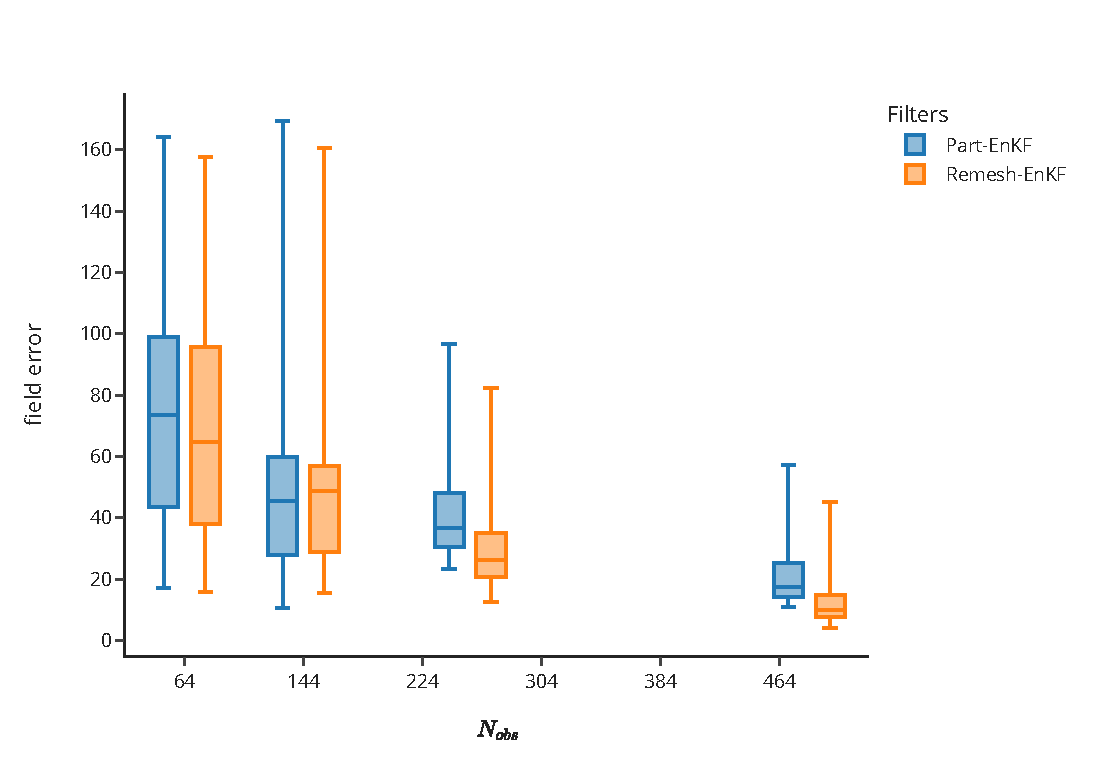
\includegraphics[width=\linewidth]{./images/app2d/final/MSE_nobs_box.pdf}
		\caption{Box plots of the state error w.r.t. $N_{\text{obs}}$.}
		\label{fig:nobs_1}
	\end{subfigure}
	\begin{subfigure}{0.49\linewidth}
		\centering
		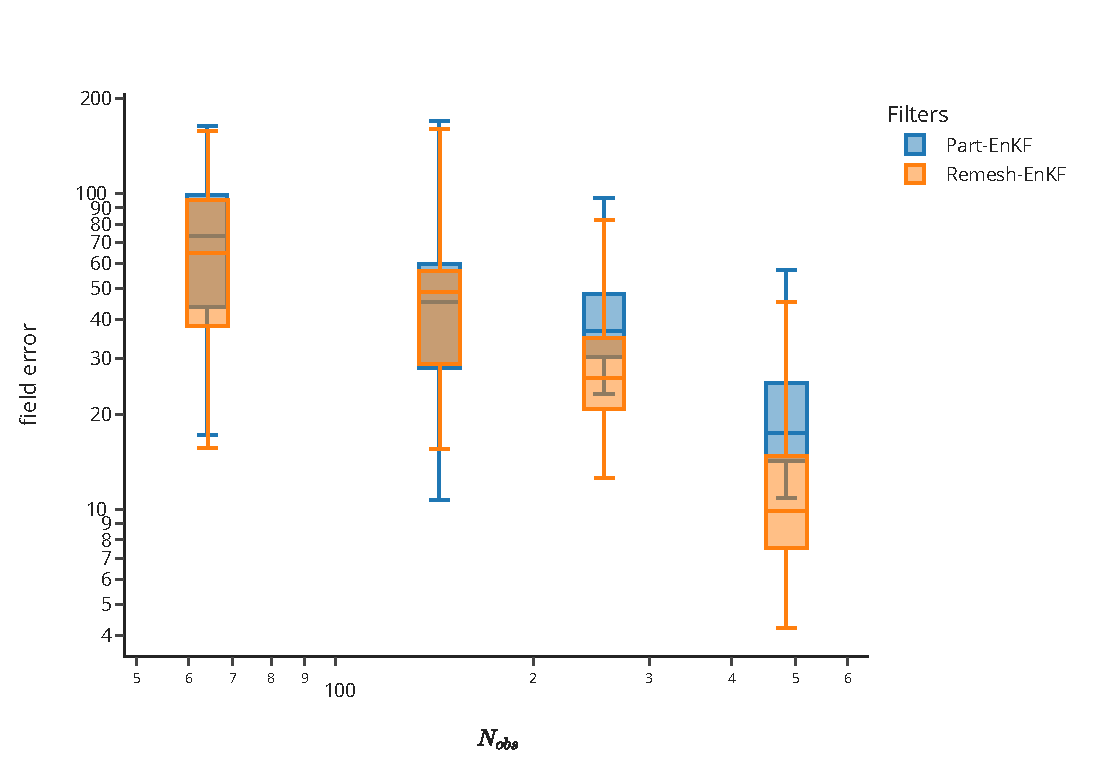
\includegraphics[width=\linewidth]{./images/app2d/final/MSE_nobs_box_log_log.pdf}
		\caption{Box plots of the state error w.r.t. $N_{\text{obs}}$.}
		\label{fig:nobs_2}
	\end{subfigure}
	\label{fig:nobs}

	\label{fig:assim_params}
\end{figure}



\subsubsection{Error with respect to simulation parameters}

To better understand the differences, let us now turn to the evolution of the error with respect to particle discretization parameters. For the Part-EnKF, remember that each member has its own particle discretization that flows according to the dipole direction and velocity. Each analyzed member's solutions are then respectively projected on their member discretization. However, this scheme could introduce different sources of error. First, due to particle irregularity in the particle distribution, severe approximation was introduced, which led to errors between the analyzed and the approximated solution. Even more seriously, certain parts of the solution may vanish as no particle in the support can interpolate it. This effect could be appreciated on several samples of the ensemble where the analysis is projected on a non-conforming particle discretization. For instance, we analyzed the first assimilation step of one member for the different filters. If the analyzed field is known over the space domain, we observed in Figure~\ref{fig:assim_member} that the Remesh-Filter and Part-Grid-EnKF are only able to interpolate the entire solution. The Part-EnKF is not entirely able to interpolate the solution with the forecast member discretization.
Moreover, some distortions observed in the particle distribution are not in line with the analyzed field flow. These remarks are more critical when the forecast step is longer, leading to high errors, or when the size of the support is lower. Moreover, the approximation of Section~\ref{regressionOperator} will introduce the approximation error function of the size of the particles. For instance, the particle will not conserve the total circulation due to a quadrature error, which is the opposite case for the Remesh-EnKF filter.

\begin{figure}[h!]
	\centering
	\begin{subfigure}{0.32\textwidth}
		\centering
		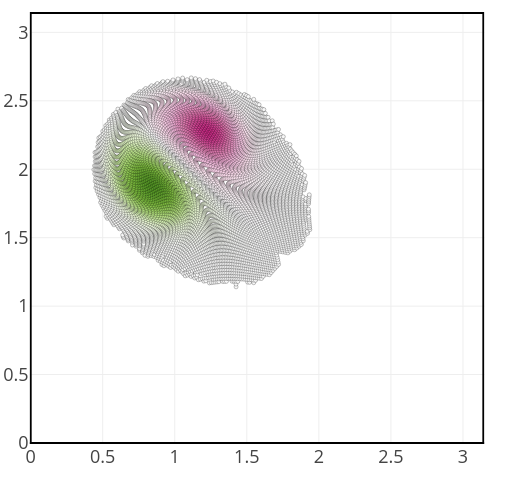
\includegraphics[width=\linewidth]{./images/app2d/assim_member_forecast.png}
		\caption{Forecast member discretization.}
	\end{subfigure}
	\hfill
	\begin{subfigure}{0.32\textwidth}
		\centering
		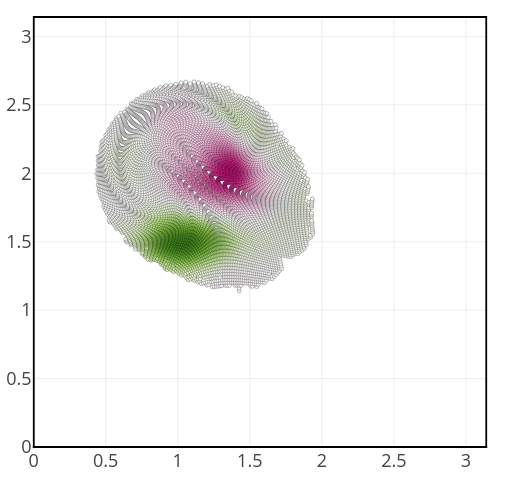
\includegraphics[width=\linewidth]{./images/app2d/assim_member_ppf.png}
		\caption{Part-EnKF analyze discretization.}
	\end{subfigure}
	\hfill
	\begin{subfigure}{0.32\textwidth}
		\centering
		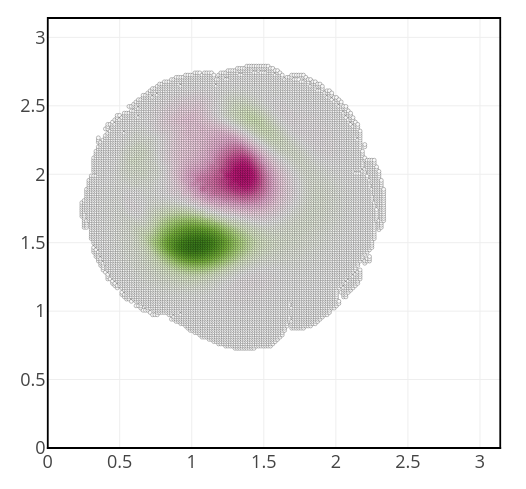
\includegraphics[width=\linewidth]{./images/app2d/assim_member_rmf.png}
		\caption{Remesh-EnKF analyze discretization.}
	\end{subfigure}
	\caption{Assimilation of one member with a forecast discretization unadapted to the analyses solution. The forecast discretization used by the Part-EnKF does not always support approximation for the analyses and introduces discretization errors.}
	\label{fig:assim_member}
\end{figure}

To evaluate the effect of the size of the support, we varied the value of $\epsilon_{\omega}$. We have seen in Figure~\ref{fig:eps_effect} that this parameter affects the number of particles and, thus, the size of the support. In Figure~\ref{fig:cuttoff}, we observe high disparities between the two filters. However, the error stabilizes rapidly by decreasing the threshold. These findings suggest an impact on the threshold and, thus, the particle support for the Part-EnKF. By contrast, Remesh-EnKF is less sensible. As a consequence, it only thresholds low values in the analyzed solutions.

\begin{figure}[h!]
	\centering

	\begin{subfigure}{0.48\textwidth}
		\centering
		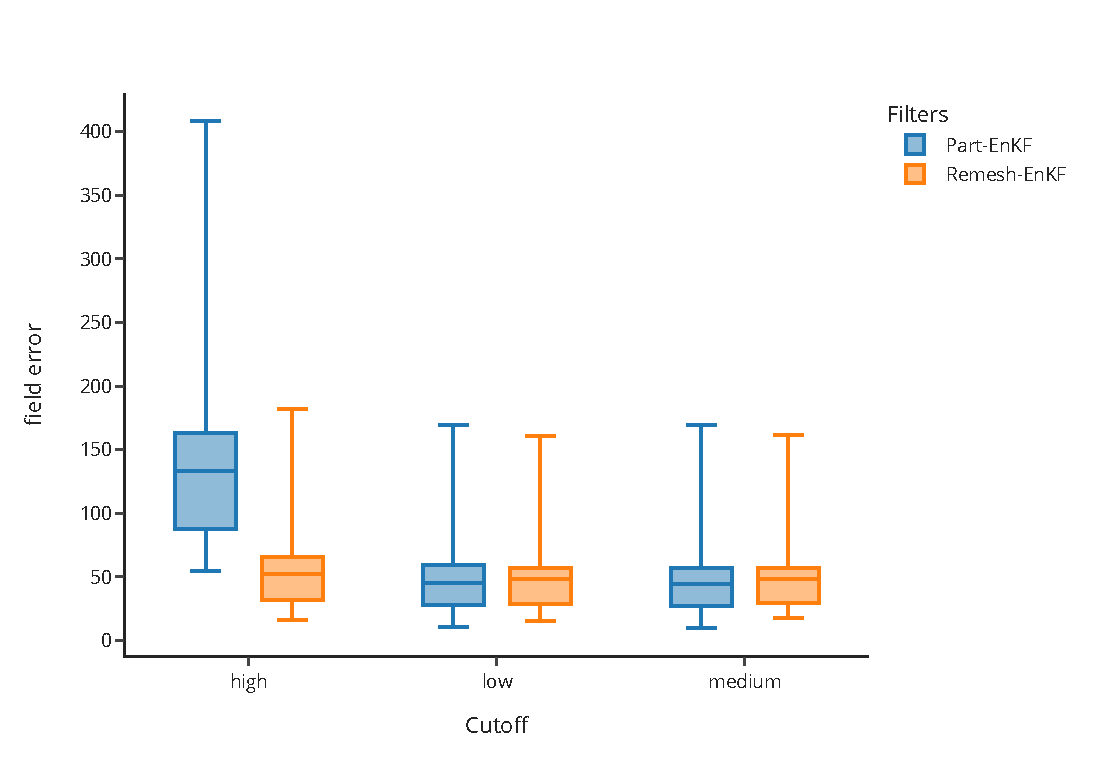
\includegraphics[width=\linewidth]{./images/app2d/final/MSE_cutoff_box.pdf}
		\caption{state error w.r.t. $\varepsilon_{\omega}$. The High, low, and medium cutoff correspond respectively to $\varepsilon_{\omega} = 0.1, 1.e^{-6}$ and $0.01$.}
		\label{fig:cuttoff}
	\end{subfigure}
	\hfill
	\begin{subfigure}{0.48\textwidth}
		\centering
		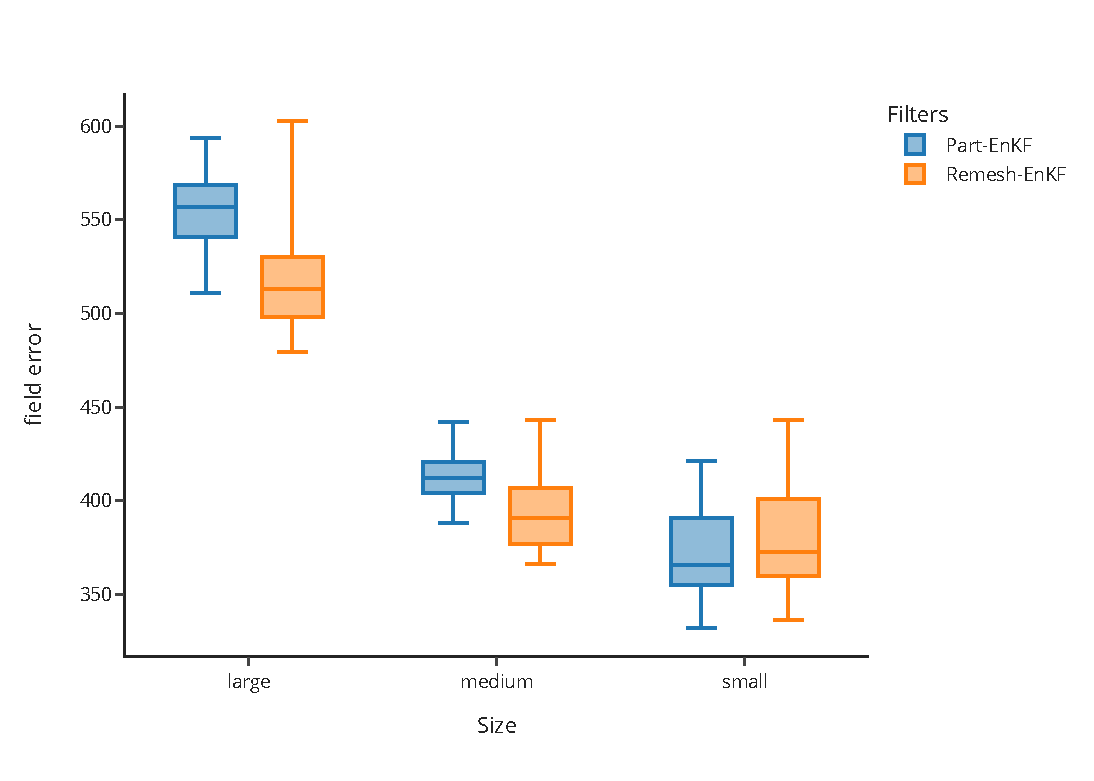
\includegraphics[width=\linewidth]{./images/app2d/final/MSE_size_box.pdf}
		\caption{state error w.r.t. $d_p$. The large, medium, and low sizes correspond to $d_p = 0.0327, 0.0245$, and $0.0123$.}
		\label{fig:np}
	\end{subfigure}

	\caption{Error box plots for simulation parameters. The effect of $\varepsilon_{\omega}$ on the error is particularly observed on high value. The Part-EnKF error is strongly linked to $d_p$ through the particle approximation error.}
	\label{fig:simu_parameters_error}
\end{figure}

In terms of particle size $d_p$, we evaluate its effect on the assimilation. In this section, we have used the regression operator defined in Section~\ref{regressionOperator} for Part-EnKF. This choice has been motivated to accelerate the update process.
in Figure \ref{fig:np}. We observe that the error for Part-EnKF and Part-Grid-EnKF increases proportionally with $d_p$ as for the approximation error. This high error confirmed, in that case, the high effect of the particle approximation for Part-EnKF. In contrast, the Remesh-EnKF error is relatively low, taking advantage of a high-order projection interpolation scheme. Using a regression operator to approximate the analyzed solution should alleviate this effect provided other particle discretization considerations (distortion, support size) as illustrated in Part~\ref{App_1D} and the choice of an adequate penalty coefficient to succeed in approximating the solution.


This discussion pointed out the high dependency of the Part-EnKF on particle discretization. The particle discretization of a member may be too far from the solution support of particles. This opens the question of the choice or modification of the particle discretization. As suggested in Part~\ref{App_1D}, an error estimation could be introduced to choose between the different filters. On the other hand, other approaches could be to select the member with the maximum likelihood estimate to approximate the solution. This proposition has to be evaluated because it could considerably reduce the variance of the ensemble. Finally, an alignment of particles might be introduced to better fit the analyzed solution.

\newpage


% % !TEX root = main.tex

\section{Conclusion}
In this study, we introduce a novel framework that combines a sequential ensemble data assimilation approach with particle-based models. Specifically, we have developed two novel Ensemble Kalman Filter schemes dedicated to meshfree simulations. These formulations depend either on an update of the particle quantities or on remeshing the particle discretization on a common ensemble grid.

We proposed two update strategies relying on a update matrix that does not directly depend on the state discretization. The first strategy, named Remesh-EnKF is based on the projection of every member onto a new common discretization of particles. The second strategy, named Part-EnKF evaluates the analysis field at particle locations to update the particle quantities.

The different classes have been initially tested on a one-dimensional example and compared with an Eulerian representation of the solution. The results show comparability among the different filters, except for some configurations of the Part-EnKF. It has been demonstrated that provided the support of the particles is consistent with the analysis solution, the filters yield similar results. However, in cases where the support deviates from the analysis field, members diverge. Increasing the support for the solution is necessary.

A two-dimensional case has also been tested, particularly to assess nonlinear advection schemes with various configurations. We observe good agreement among the different filters. However, this time, the particle approximation is predominant in the Part-EnKF.
Both strategies offer several derivations. Remesh-EnKF is mainly dependent on the redistribution kernel to obtain the new regularly spaced particle set. Part-EnKF could be extended because it is highly flexible in defining the new set of particles for each member. This tuning is essential, as we have highlighted the issue of the non-conforming support of the forward particle position with the analysis.

Several methodologies to introduce new particles or change the previous ones could be explored, particularly at the edge of the distribution.
For the sake of simplicity, we advocate generating a new set of particles with a regular spacing for any member encountering difficulties in accurately reconstructing the analysis field.
Another alternative is to update the positions of the particles in addition to the intensities instead of only changing the intensities. In this way, the error due to a misfit of alignment or approximation could be avoided. These type of adaptation could be derived from optimal transport scheme~\cite{bocquet_bridging_2023} or correction of the background ensemble alignment with the observation~\cite{ravela_data_2007,rosenthal_displacement_2017} .

\newpage
% !TEX root = main.tex

\appendix
\section{Stochastic Ensemble Kalman Filter}~\label{appendix:enkf}

We define the matrix of states and the matrix of anomalies $\X_f = [\state^1, \dots, \state^N]$, $\annomX_f$ whose columns are the member states and the normalized anomalies.

\begin{equation*}
    \annomX_f = \frac{1}{\sqrt{N - 1}}(\X_f - \overline{\state}_f \bm{1}^T),
\end{equation*}where$\bm{1} \in \mathbb{R}^N$ is a vector of one.

Respectively the matrix of observation and observation anomalies are $\mathcal Y_f = [\mathcal{H}(\state^1_f), \dots, \mathcal{H}(\state^N_f)]$, $\annomY_f$ where columns are

\begin{equation*}
    \annomY_f = \frac{1}{\sqrt{N - 1}} \left(\mathcal Y_f - \overline{\obs}_f \bm{1}^T \right) \quad \text{with} \quad \overline{\obs}_f = \frac{1}{N} \sum_{j=1}^{N} \mathcal{H}(\state^j_f).
\end{equation*}

The ensemble defines the covariance between states and observations $\Cov \bm H^T$, the covariance between observations $\Cov \bm H^T$, and $\tilde{\bm{K}}$

\begin{eqnarray*}
    \Cov \bm H^T &=& \frac{1}{N - 1} \sum_{i = 1}^{N} {(\state^i_f - \overline{\state}_f)}^T {\left[ \mathcal{H}_k(\state^i_f) - \overline{\bm{y}}_f\right]}^T = \annomX_f \annomY_f^T, \\
    \bm H \Cov \bm H^T &=& \frac{1}{N -1} \sum_{i = 1}^{N}\left[ \mathcal{H}_k(\state^i_f) - \overline{\bm{y}}_f\right] {\left[ \mathcal{H}_k(\state^i_f) - \overline{\bm{y}}_f\right]}^T = \annomY_f \annomY_f^T,\\
    \tilde{\bm{K}} &=& \Cov \bm H^T{(\bm H \Cov \bm H^T + \bm R)}^{-1} = \annomX_f \annomY_f^T {(\annomY_f \annomY_f^T + \bm R)}^{-1}.
\end{eqnarray*}

This observation matrix-free implementation rely on the secant method approximation $\mathcal{H}(\state^i_f - \overline{\state}_f) \approx \predi - \overline{\obs}_f$.
The forecast is then update to a posterior ensemble ${[\state^i_a]}_{i=1}^{N}$ such as

\begin{equation} \label{enkf_formula}
    \mstate_a = \mstate_f + \tilde{\bm{K}} ( \mdata - \mpred),
\end{equation}where ${[\mdata]}^i = \obs + \bm{\varepsilon}^i$ is the perturbed observation with $\bm{\varepsilon}^i \sim \mathcal{N}(\bm{0}, \bm R) $, $\tilde{\bm{K}}$ the ensemble Kalman gain matrix and $( \mdata - \mpred)$ the innovation term.
The forecast step is then applied to the analyzed ensemble until the following observation.
Based on this formulation, we can deduce a correction formula only based on the member's predictions and observations.

We can rewrite the classical update formula using the previous anomaly matrices.

\begin{equation*}
    \mstate_a = \mstate_f + \annomX_f \annomY_f^T {({\annomY_f \annomY_f^T + \bm R})}^{-1}(\mdata - \mpred)
\end{equation*}

We reformulate the correction term by remarking that $ \bm{1}^T  \annomY_f^T = \bm{0}$. We define $\Fcorr$, the correction matrix that gives the update in terms of linear combinations of the forward states

\begin{equation*}
    \mstate_a = \mstate_f + \mstate_f \Fcorr, \quad \Fcorr = \frac{1}{\sqrt{N - 1}}\annomY_f^T {(\annomY_f \annomY_f^T + \bm R)}^{-1}(\mdata - \mpred).
\end{equation*}.

using the Sherman-Morrison-Woodbury formula we obtain

\begin{equation*}
    \Fcorr = \frac{1}{\sqrt{N - 1}} {(\bm I_N + \annomY_f^T\bm R^{-1}\annomY_f)}^{-1}\annomY_f^T \bm R^{-1} (\mdata - \mpred).
\end{equation*}
\section{Moment conservation of particle discretization}~\label{appendix:moment_conservation}

The $m$-th moment of a particle distribution is defined as the quantity $\sum_{p} z_p^{\alpha} \bm{U}_p$.

First, we see that the partition of unity is required

\begin{equation}~\label{eq:unity1}
    \sum_{I \in \Lambda} W\left(\frac{z - z_I}{\ell_I}\right) = 1 ,\quad z \in \Omega
\end{equation}~due to the final particle arrangement $\mathcal{P'}$ on a grid of size $d_p$, it leads to the following property

\begin{equation}~\label{eq:unity2}
    \sum_{p'\in\mathcal P'} W\left(\frac{z - z_{p'}}{\ell_I}\right) = \frac{V_I}{V_p'},\quad z \in \Omega.
\end{equation}.

Attention should be focused on the border. Extending the domain with "ghost" particles or nodes allows for verification of properties within $\Omega$.

This property is the necessary condition for the conservation of the first moment. Primarily for the assignment

\begin{gather}
    \begin{align*}
        \sum_{I \in \Lambda} \bm u_I V_I & = \sum_{p \in \Lambda} \bm U_p  W \left(\frac{z_I - z_p}{\ell_I} \right)                                                           & \\
                                         & = \sum_{p \in \mathcal P} \bm U_p \sum_{I \in \Lambda} W \left(\frac{z_I - z_p}{\ell_I} \right) = \sum_{p \in \mathcal P} \bm U_p. &
    \end{align*}
\end{gather}~using the property \eqref{eq:unity1}. Secondary, for the interpolation process

\begin{gather}
    \begin{align*}
        \sum_{p' \in \mathcal P'} \bm U_{p'} = \sum_{p' \in \mathcal P'} \bm u_g(z_{p'}) V_{p'} & = \sum_{p' \in \mathcal P'} V_{p'} \sum_{I \in \Lambda} \bm u_I W \left(\frac{z_{p'} - z_I}{\ell_I}\right)                                                &   \\
                                                                                                & =  \sum_{I \in \Lambda} \bm u_I  V_{p'}\sum_{p' \in \mathcal P'} W \left(\frac{z_{p'} - z_I}{\ell_I}\right)                                               &   \\
                                                                                                & =  \sum_{I \in \Lambda} \frac{V_I}{V_p'} V_{p'} \bm u_I =                            \sum_{I \in \Lambda} \bm u_I V_{I} = \sum_{p \in \mathcal P} \bm U_p & ,
    \end{align*}
\end{gather}~using equation~\eqref{eq:unity2}.

It can be shown moreover that if for $1 \leq |\alpha| \leq m - 1$, $W$ satisfies,

\begin{equation}
    \sum_{I \in \Lambda} {(\bm z-\bm z_I)}^\alpha W \left(\frac{\bm z - \bm z_I}{\ell_I} \right) = 0, \label{eq:momentProperty}
\end{equation}

The regridding procedure will be ordered at $m$. Equivalently, the previous equality lead, for $0 \leq |\alpha| \leq m - 1$, to
\begin{equation*}
    \sum_{I \in \Lambda} \bm z_I^\alpha W \left(\frac{\bm z_p - \bm z_I}{\ell_I} \right) = \bm z^\alpha,
\end{equation*}~obtained by developing ${(\bm z-\bm z_q)}^\alpha$ and using a recurrence on previous orders. This means that the interpolation is exact for polynomials of degrees less or equal to $m-1$ or that the moment of order $m-1$ is conserved.

\section{Parameters}~\label{appendix:simulation-parameters}

\subsection{One dimension problem}
\begin{table}[htbp]
    \centering
    \caption{Ensemble generation variables}
    \begin{tabular}[t]{|l|l|}
        \hline
        Variables                   & Distributions                              \\
        \hline
        Gaussian mean               & $Z_m \sim  \mathcal{N}(\meanZm, \sigmaZm)$ \\
        Gaussian standard deviation & $S_m \sim\mathcal{U}(\smLow, \smUp)$       \\
        velocity                    & $v \sim \mathcal{N}(\vmean, \vstd)$        \\
        diffusion                   & $D \sim \mathcal{U}(\Dlow, \Dup)$          \\
        \hline
    \end{tabular}
    \label{tab:ens_gen_1d}
\end{table}

\subsection{Two dimension problem}
\begin{table}[htbp]
    \centering
    \caption{Reference parameters}
    \begin{tabular}[t]{|l|l|}
        \hline
        Parameters            & Values                                                       \\
        \hline
        reference viscosity   & $v_{\text{ref}} = 0.001$                                     \\
        reference orientation & $\theta_{\text{ref}}  = \frac{7 \pi}{8} (\text{rad.})$       \\
        barycenter position   & $\bm{z}_{\text{ref}} = \left[\frac\pi2, \frac\pi2 \right]^T$ \\
        translation velocity  & $U_{\text{ref}} = 0.25$                                      \\
        \hline
    \end{tabular}
    \label{tab:ref}
\end{table}

\begin{table}[htbp]
    \centering
    \caption{Nominal assimilation and simulation parameters}
    \begin{tabular}[t]{|l|l|}
        \hline
        Parameters                      & Values                                 \\
        \hline
        time step                       & $dt = 0.005$                           \\
        final time                      & $t_f =10$                              \\
        std. observation                & $\sigma_{obs} =  5.0e^{-2}$            \\
        vorticity threshold             & $\varepsilon_{\omega} = 1.0e^{-4}$     \\
        particle characteristic length  & $dp = \frac{pi}{256} \approx 0.01227 $ \\
        smoothing length                & $h = 2.0 dp$                           \\
        number of assimilation          & $N_{\text{assim}} = 10$                \\
        ensemble size                   & $N_{\text{ens}} = 32$                  \\
        number of observation           & $N_{\text{obs}} = 12^2 = 144$          \\
        grid discretization             & $N_{\text{grid}} = 65^2 = 4225$        \\
        number of remeshing by forecast & $N_{\text{remesh}} =  2 $              \\
        \hline
    \end{tabular}
    \label{tab:simu_2d}
\end{table}

\begin{table}[htbp]
    \centering
    \caption{Ensemble generation variables}
    \begin{tabular}[t]{|l|l|}
        \hline
        Variables   & Distributions                                                                                                           \\
        \hline
        radius      & $R \sim \cN(1.0, 0.05^2)$                                                                                               \\
        orientation & $\theta \sim \cU\left(\pi, \frac\pi2 \right) (\text{rad.}) $                                                            \\
        barycenter  & $z_{\text{mean},x} \sim \cN\left(\frac\pi2,0.1^2\right), \quad z_{\text{mean},y} \sim \cN\left(\frac\pi2,0.1^2\right) $ \\
        velocity    & $U \sim \cU(0, 0.5^2) $                                                                                                 \\
        viscosity   & $v \sim \cN(0.0015, 0.0005^2)$                                                                                          \\
        \hline
    \end{tabular}
    \label{tab:ens_dipole}
\end{table}

\newpage
% \section*{References}

\bibliography{C:/Users/md266594/mar-dvd-thesis/articles/new_part_enkf/biblio}

% \nocite{*}
% \printbibliography

\end{document}